%%%%%%%%%%%%%%%%%%%%%%%%%%%%%%%%%%%%%%%%%
% Их сургуулийн оюутны тезис  
% LaTeX Загвар
% Version 2.3 (25/3/16)
%
% Энэ загвар нь дараах сайтаас авсан загварын монгол хувилбар юм.
% http://www.LaTeXTemplates.com
%
% Version 2.x major modifications by:
% Vel (vel@latextemplates.com)
%
% Анхдагч загварын эх үүсвэр:
% Steve Gunn (http://users.ecs.soton.ac.uk/srg/softwaretools/document/templates/)
% Sunil Patel (http://www.sunilpatel.co.uk/thesis-template/)
%
% Загварын лиценз:
% CC BY-NC-SA 3.0 (http://creativecommons.org/licenses/by-nc-sa/3.0/)
%
%%%%%%%%%%%%%%%%%%%%%%%%%%%%%%%%%%%%%%%%%

%-------------------------------------------------------------------------------
%	PACKAGES AND OTHER DOCUMENT CONFIGURATIONS
%-------------------------------------------------------------------------------

\documentclass[
11pt, % Баримтын фонтын хэмжээ, сонголт: 10pt, 11pt, 12pt
oneside, % Хоёр талаар хэвлэж үдэхээр тохируулсан. Нэг тал бол комментыг арилга
%chapterinoneline,% Нэг мөрөнд бүлгийн дугаар, нэрийг гаргах
english, % babel багцын хэлний тохиргоо
singlespacing, % Мөр хоорондын зай. Сонголтууд: singlespacing, onehalfspacing, doublespacing
%draft, % Ноорог горимд шилжихийн тулд комментыг арилга(зураг, холбоос, hboxes гарахгүй)
nolistspacing, % Хэрэв мөр хоорондын зай onehalfspacing эсвэл doublespacing бол, жагсаалтын мөр хоорондын зайг single болгохын тулд комментыг арилга
%liststotoc, % Зураг/хүснэгт/бусад жагсаалтыг гарчигт оруулахын тулд комментыг арилга
%toctotoc, % Uncomment to add the main table of contents to the table of contents
%parskip, % Параграф хооронд зай оруулахын тулд комментыг арилга
%nohyperref, % hyperref багцыг ачаалахгүй бол комментыг арилга
%headsepline, % Толгой мөрийн доогуур шугам татахын тулд комментыг арилга
]{MUST-Thesis} % Энэ класс файл нь баримтын бүтцийг тодорхойлно

%-------------Монгол хэлний драйвер, Times New Roman фонд----------------------------------------- 
\usepackage[utf8]{inputenc} % Олон улсын тэмдэгт оруулахад хэрэгтэй
\usepackage[T2A]{fontenc} % Олон улсын тэмдэгтийн гаралтын кодчилол
\usepackage[mongolian]{babel}

%----------------Жагсаалтын дугаарлалтыг өөрчлөх нэмэлт багц ------------------------------------
\usepackage{enumitem}

%-------------Хүснэгт үүсгэх, зохион байгуулахтай холбоотой багцууд--------------------------------
\usepackage{titlesec}
\usepackage[table]{xcolor}
\usepackage{rotating} % эргүүлэх
\usepackage{multirow}

\usepackage{longtable}

\usepackage{tabularx}
\newcolumntype{Y}{>{\raggedleft\arraybackslash}X}
\newcolumntype{Z}{>{\centering\arraybackslash}X}

\usepackage{tcolorbox}
\usepackage{array}
\usepackage{colortbl}
\tcbuselibrary{skins}

\tcbset{tab2/.style={enhanced,fonttitle=\bfseries,fontupper=\footnotesize\rmfamily,
		colback=white,colframe=black,colbacktitle=white,
		coltitle=black,center title,sharp corners=all}}

\newcounter{tblerows}
\expandafter\let\csname c@tblerows\endcsname\rownum


%---------------математик томъёо дүрслэлийн багц----------
\usepackage{amsmath,amssymb}
\usepackage{mathtools, nccmath}

% ------------текстийн хажууд зураг оруулах, дэд зурагнуудыг ялгаж нэрлэх нэмэлт багц----------------------------
\usepackage{wrapfig}
\usepackage{subcaption}

%-------------LaTeX командаар зураг зурах багц ---------------------------------------------------------------
\usepackage{pgf}
\usepackage{tikz} % зураг зурах
\usetikzlibrary{shapes,arrows,automata,positioning,fit,calc,patterns}
\usepackage{pgfplots}
\pgfplotsset{compat=1.18}
\usepackage{xcolor}

%------------цаасны өнгө солих багц: нүүр хуудсыг цайвар цэнхэр (LigthBlue) , бүлэг бүрийн эхлэл хуудсыг шаргал (Beige) өнгөтэй болгож болно.-----
%----------- өөр өнгө хүсвэл өнгөний кодоо өөрчилж өгөөрэй--------------------------------------------
\usepackage{pagecolor}
\definecolor{LigthBlue}{RGB}{102,255,255}
\definecolor{Beige}{RGB}{255,220,180}

%----------- програмын кодыг таньж түлхүүр үгнүүдийг өнгөөр ялгаж хэвлэх тохиргоо-----------------------
%----------- түлхүүр үгийг Оливын ногоон (OliveGreen), тайлбар comment ийг бүдэг хөх (CadetBlue), кодын арын фонийг цайвар саарал (LigthlightGray) өнгөөр тус тус тохируулсан. Хүсвэл өнгөний кодыг өөрчлөөрэй------------------------------- 

\definecolor{OliveGreen}{cmyk}{0.64,0,0.95,0.40}
\definecolor{CadetBlue}{cmyk}{0.62,0.57,0.23,0}
\definecolor{lightlightgray}{gray}{0.9}

%---------- програмын кодыг таньж хэвлэх тохиргоо -----------------------------
\usepackage{listingsutf8}
\renewcommand{\lstlistingname}{Эх код} % Програмын эх код хэвлэх
\lstset{
language={[x86masm]Assembler},          % Code langugage  [x86masm]Assembler C VHDL Phyton 
basicstyle=\ttfamily,                   % Code font
keywordstyle=\color{OliveGreen},        % Keywords font ('*' = uppercase)
commentstyle=\color{CadetBlue},         % Comments font
numbers=left,                           % Line nums position
numberstyle=\tiny,                      % Line-numbers fonts
stepnumber=1,                           % Step between two line-numbers
numbersep=5pt,                          % How far are line-numbers from code
backgroundcolor=\color{lightlightgray}, % Choose background color
frame=none,                             % A frame around the code
tabsize=2,                              % Default tab size
captionpos=t,                           % Caption-position = bottom
breaklines=true,                        % Automatic line breaking?
breakatwhitespace=false,                % Automatic breaks only at whitespace?
showspaces=false,                       % Dont make spaces visible
showtabs=false,                         % Dont make tabls visible
columns=flexible,                       % Column format
morekeywords={__global__, __device__},  % CUDA specific keywords
extendedchars=true,                     % Монгол тэмдэгт зөвшөөрөх
inputencoding=utf8,                     % UTF-8 кодчилол
}

\usepackage[autostyle=false]{csquotes} % Ном зүйд хэлнээс хамаарсан хашилт оруулахад хэрэгтэй

%-----------------Ном зүй үүсгэх -------------------------------------
\usepackage[backend=biber,natbib=true,sorting=none,sortcites]{biblatex} % Ном зүйд bibtex -г ашиглах
\addbibresource{references.bib} % Ном зүйн файл

%----------------дахин ашиглах командууд (бүх бүлгийн өмнө тодорхойлох) -------------------
\newcommand{\keyword}[1]{\textbf{#1}}
\newcommand{\tabhead}[1]{\textbf{#1}}
\newcommand{\code}[1]{\texttt{#1}}
\newcommand{\file}[1]{\texttt{\bfseries#1}}
\newcommand{\option}[1]{\texttt{\itshape#1}}

%----------------хэвлэмэл файлд монгол хэлээр бичих зарим командууд -----------------------
\newcommand{\authorshipname}{Зохиогчийн эрх хамгаалал}
\newcommand{\abbrevname}{Товчилсон үгс}
\newcommand{\constantsname}{Физик тогтмолууд}
\newcommand{\symbolsname}{Таних тэмдэгтүүд}
\newcommand{\acknowledgementname}{Талархал}
\newcommand{\abstractname}{Хураангуй}
\newcommand{\conclusionname}{Дүгнэлт}
 
%-------------------------------------------------------------------------------
%	THESIS INFORMATION
%-------------------------------------------------------------------------------
% -------------- Төгсөлтийн ажлын сэдвийг монгол, англи хэлээр, гүйцэтгэгч оюутны бүтэн болон товчилсон нэр, код, e-mail хаягийн мэдээлэл ----------------
\thesistitle{Үүлэн орчинд суурилсан спорт заалны цаг захиалгын 3 давхаргат системийн загварчлал, хэрэгжилт} % Таны ажлын нэр, нүүр болон хураангуй хуудсанд ашигласан. Өөр газарт бол \ttitle командыг хэрэглэнэ
\thesistitleeng{Design and Implementation of a Three-Tier Sports Hall Booking System Based on Cloud Environment} % Таны ажлын нэр, нүүр болон хураангуй хуудсанд ашигласан. Өөр газарт бол \ttitleng командыг хэрэглэнэ
\thesistype{Бакалаврын төгсөлтийн ажил} % нүүр хуудсанд ашиглана. Дурын газарт бол \thesisname командыг хэрэглэнэ
\authorshort{М.Түвшинжаргал} % Таны товч нэр, нүүр болон хураангуй хуудсанд ашигласан. Дурын газарт бол \shortname командыг хэрэглэнэ
\authorlong{М.Түвшинжаргал} % Таны бүтэн нэр, нүүр болон хураангуй хуудсанд ашигласан. Дурын газарт бол \longname командыг хэрэглэнэ
\authorcode{В221940619} % Таны оюутны код, үзлэгийн хуудсанд ашигласан.  Дурын газарт бол \studentcode командыг хэрэглэнэ
\authormail{} % Таны хаяг, хураангуйд ашигласан. Өөр газарт бол \mailaddress командыг хэрэглэнэ
\authorphone{} % Таны утасны дугаар, хураангуйд ашигласан. Өөр газарт бол \phonenum командыг хэрэглэнэ
\keywords{Flutter, Firebase, Node.js, Docker, AWS, цаг захиалга, спорт заал, үүлэн орчин} % Түлхүүр үгс, хураангуйд ашигласан. Дурын газарт бол \keywordnames командыг хэрэглэнэ

% -----------Удирдагч, зөвлөх, шүүмжийн багшийн мэдээлэл ---------------------
% --багшийн нэрийг Овгийн эхний үсгийг товчилж, бүтэн нэрээр бичнэ.-----------
% --Багшийн цол зэргийг жижиг үсгээр, бүтэн үгээр Нэрний урд бичнэ.----------
% -- багшийн мэргэжлийн зэрэг бакалавр, магистр, доктор гэсэн 3 шатлалтай----
% --доктор зэргийг боловсролын доктор бол доктор (Ph.D), ШУ-ны доктор бол доктор (Sc.D)  гэж ялгаж бичнэ. 
% -- магистр зэргийг магистр гэнэ. Ms.C гэсэн товчлол ашиглахгүй ------------
% -- ШУТИС-ийн багшийн цол дэд профессор, профессор гэсэн 2 шатлалтай. цолыг зэргийн ард таслалаар зааглаж бичнэ. товчлохгүй. Жнь. доктор (Ph.D), профессор Б.Зоригтбаатар

\supervisor{Доктор Д.Эрдэнэтуяа} % Удирдагчийн нэр, нүүр хуудсанд ашиглана. Дурын газарт бол \supname командыг хэрэглэнэ
\reader{Доктор Б.Намжилдорж} % Шүүмжлэгчийн нэр, Дурын газарт бол \readname командыг хэрэглэнэ
\readeraddress{Өмнөговь Технологийн Дээд Сургууль, Мэдээллийн технологийн тэнхим} % Шүүмжлэгчийн ажлын газар, Дурын газарт бол \readaddress командыг хэрэглэнэ
\advisorA{} % Зөвлөгчийн нэр, Дурын газарт бол \advicenameA командыг хэрэглэнэ
%\advisorB{магистр Н.Чулуунбаатар} % Зөвлөгчийн нэр, Дурын газарт бол \advicenameB командыг хэрэглэнэ

%---------- мэргэжил, хөтөлбөр, харьяалагдах салбар, сургуулийн мэдээлэл ------------
% -- ижил мэргэжлийн оюутнуудад энэ хэсгийн мэдээлэл ижил байна. 

\degreeindex{D061304} % Мэргэжлийн индекс, нүүр болон хураангуй хуудсанд ашигласан. Өөр газарт бол \degreeid командыг хэрэглэнэ
\degree{Мэдээллийн технологи} % мэргэжлийн нэр, нүүр болон хураангуй хуудсанд ашигласан. Өөр газарт бол \degreename командыг хэрэглэнэ
\program{Мэдээллийн технологи} % хөтөлбөрийн нэр, нүүр болон хураангуй хуудсанд ашигласан. Өөр газарт бол \programname командыг хэрэглэнэ
\subject{} % Таны салбар, одоогоор ашиглаагүй. Дурын газарт бол \subjectname командыг ашиглана
\department{Мэдээллийн технологийн тэнхим} % Сургууль/тэнхмийн нэр, нүүр болон хураангуй хуудсанд ашигласан. Дурын газарт бол\deptname командыг хэрэглэнэ
\deptchair{} % Тэнхим/эрхлэгчийн нэр, нүүр болон хураангуй хуудсанд ашигласан. Дурын газарт бол\chairname командыг хэрэглэнэ
\group{} % Судалгааны баг/тэнхмийн нэр, нүүр хуудсанд ашигласан. Дурын газарт бол \groupname командыг хэрэглэнэ
\faculty{Мэдээллийн Технологийн Тэнхим} % Салбар сургууль/факультетийн нэр, нүүр болон хураангуй хуудсанд ашигласан. Дурын газарт бол \facname командыг ашиглана
\university{Өмнөговь Технологийн Дээд Сургууль} % Их сургуулийн нэр ба веб хаяг. Дурын газарт бол \univname командыг хэрэглэнэ 

\hypersetup{pdftitle=\ttitle} % Pdf файлын гарчиг
\hypersetup{pdfauthor=\shortname} % Pdf файлын зохиогчийн нэр
\hypersetup{pdfkeywords=\keywordnames} % Pdf файлын түлхүүр үгс
\hypersetup{allcolors=black} % Pdf файлын бүх холбоос хар өнгөтэй

\begin{document}

\frontmatter % Агуулгын өмнөх хуудас дугаарлалт: i, ii, iii, iv... г.м.

\pagestyle{plain} % Тезисийн загварыг дуудах хүртэлх толгой мөрийн суурь загвар

%-------------------------------------------------------------------------------
%	TITLE PAGE
%-------------------------------------------------------------------------------

\begin{titlepage}
%\pagecolor{LigthBlue} % нүүр хуудас өнгөтэй болгохыг хүсвэл comment-ийг авна.
\begin{center}

{\scshape\LARGE \univname\par} % Их сургуулийн нэр
{\scshape\Large \facname\par}\vspace{1 cm} % Их сургуулийн нэр

\begin{figure}[!htbp]
\centering

\includegraphics[scale=1.2]{Figures/MUST_logo.png}
\end{figure}

\vspace{1cm}
\hfill \large{\longname} \\

\vspace{1.5cm}

{\huge \bfseries \ttitle\par}\vspace{0.4cm} % Тезисийн нэр

\vspace{3cm}
\textsc{\Large {\thesisname}}\\ % Тезисийн төрөл

\vfill

\large {Даланзадгад хот} \\
 
\end{center}
\end{titlepage}

%-------------------------------------------------------------------------------
%	SUBTITLE PAGE
%-------------------------------------------------------------------------------

\begin{titlepage}
\begin{center}
\pagecolor{white}
{\scshape\LARGE \univname\par} % Их сургуулийн нэр
{\scshape\Large \facname\par}\vspace{0.5cm} % Их сургуулийн нэр

\vspace{2cm}
\hfill \large{\deptname} \\

\vspace{3cm}

{\huge \bfseries \ttitle\par}\vspace{0.4cm} % Тезисийн нэр

\vspace{2cm}

\begin{minipage}[t] {0.9\textwidth}
\begin{flushleft} 
\normalsize

Мэргэжлийн индекс: \degreeid \\
Мэргэжил: \degreename \\
%Хөтөлбөр: \programname \\ [2cm]

\begin{tabular}{l l}
\emph{Удирдагч:} & {\supname} \\% Удирдагчийн нэр
\emph{Зөвлөгч:} &{\advicenameA} \\ % Зөвлөгч нарын нэрс
\emph{Гүйцэтгэгч:} &\hspace{1.4cm} {\shortname} \\ % Зохиогчийн нэр  --зэрэгцүүлэхийн тулд 1.4cm гэсэн зайг өөрчилж болно.
\end{tabular}


\end{flushleft}
\end{minipage}

\vfill

\large {Даланзадгад хот} \\
{\large 2026 он}\\ % Date

\end{center}
\end{titlepage}

  % Нүүр хуудас
%-------------------------------------------------------------------------------
%	WORK PLAN & REVIEW PAGE
%-------------------------------------------------------------------------------

%---------------------ТӨЛӨВЛӨГӨӨНИЙ ХУУДСЫН ЭХЛЭЛ--------------------------------
\begin{titlepage}
	\noindent Батлав. \deptname ын эрхлэгч:
	\begin{flushright}
		\makebox[6cm]{\dotfill} /\chairname/
	\end{flushright}
	Удирдагч:\makebox[6cm]{ \dotfill} /\supname/
	\begin{center}
		\vspace*{0.5cm}
		\textbf{{\large ТӨГСӨЛТИЙН АЖЛЫН ТӨЛӨВЛӨГӨӨ}}\\[0.5cm]
	\end{center}
	\noindent \textbf{Төгсөлтийн ажлын сэдэв:}\\
	\textbf{Монгол}: \ttitle\\
	\textbf{Англи}: \ttitleng\\

	\noindent \textbf{Төслийн зорилго}: Өмнөговь аймгийн Даланзадгад хотын спорт заалнуудын цаг захиалгыг цахимжуулах, хэрэглэгчдэд хялбар, хурдан захиалга хийх боломж олгох Flutter мобайл аппликейшн хөгжүүлэх.\\

	\noindent \textbf{Оюутны овог нэр, код}:\makebox[5cm]{ } \shortname /\studentcode/ \\
	\noindent
	\begin{tabularx}{1\textwidth}{| >{\hsize=0.2\hsize}X
			| >{\hsize=2.8\hsize}Z
			| >{\hsize=0.5\hsize}Z
			| >{\hsize=0.5\hsize}Z |}
		\hline
		\multirow{2}{*}{№} &\multirow{2}{*}{Ажлын бүлэг, хэсгийн нэр} & \multirow{2}{4em}{\centering эзлэх хувь} & \multirow{2}{5em}{\centering дуусах хугацаа} \\
		& & & \\ \hline
		\multicolumn{4}{|l|}{\parbox[l]{13cm}{Удиртгал. Оршил ба судалгааны үндэслэл}} \\  \hline
		\multirow{3}{*}{} &\multirow{3}{*}{} & \multirow{3}{*}{} & \multirow{3}{*}{} \\
		1 & \parbox[l]{9cm}{
			1.1 Үндэслэл, асуудлын тодорхойлолт \\
			1.2 Зорилго, зорилт \\
			1.3 Судлагдсан байдал, хамрах хүрээ } & 5\% & III.13 \\
		& & & \\ \hline
		\multicolumn{4}{|l|}{\parbox[l]{13cm}{Бүлэг №1. Онолын судалгаа}} \\ \hline
		\multirow{3}{*}{} &\multirow{3}{*}{} & \multirow{3}{*}{} & \multirow{3}{*}{} \\
		2 & \parbox[l]{9cm}{
			1.1 Мобайл технологи (Flutter, Dart, Firebase, AI чатбот) \\
			1.2 Бэкэнд технологи (Node.js, Express, REST API) \\
			1.3 Үүлэн технологи (Docker, AWS EC2/ECR, GitHub Actions) } & 30\% & IV.10 \\  & & & \\ \hline
		\multicolumn{4}{|l|}{\parbox[l]{13cm}{Бүлэг №2. Програм хангамжийн загварчлал ба хөгжүүлэлт}} \\ \hline
		\multirow{2}{*}{} &\multirow{2}{*}{} & \multirow{2}{*}{} & \multirow{2}{*}{} \\
		3 & \parbox[l]{9cm}{
			2.1 Програмын шаардлага ба загварчлал \\
			2.2 Frontend хөгжүүлэлт (Flutter апп, UI/UX) \\
			2.3 Backend хөгжүүлэлт (Node.js REST API, email) \\
			2.4 Өгөгдлийн сан (Firestore collection-уудын загвар) } & 30\% & V.10 \\ & & & \\ \hline
		\multicolumn{4}{|l|}{\parbox[l]{13cm}{Бүлэг №3. Хэрэгжүүлэлт}} \\ \hline
		\multirow{2}{*}{} &\multirow{2}{*}{} & \multirow{2}{*}{} & \multirow{2}{*}{} \\
		4 & \parbox[l]{9cm}{
			3.1 Үүлэн байршуулалт (Docker, AWS EC2, CI/CD) \\
			3.2 Туршилт ба үнэлгээний үр дүн } & 30\% & V.22 \\ & & & \\ \hline
		\multicolumn{4}{|l|}{\parbox[l]{13cm}{Ерөнхий дүгнэлт \hfill 5\%}} \\  \hline
	\end{tabularx}

	\vspace{0.5cm}
	Төлөвлөгөөг боловсруулсан оюутан: \makebox[3cm]{\dotfill} /\shortname/

\end{titlepage}
%---------------------ТӨЛӨВЛӨГӨӨНИЙ ХУУДСЫН ТӨГСГӨЛ ---------------------------------------------------

%---------------------ГҮЙЦЭТГЭЛИЙН ХУУДСЫН ЭХЛЭЛ ---------------------------------------------------
\newpage

\begin{titlepage}

	\begin{center}

		\vspace*{2cm}
		\textbf{{\large ТӨГСӨЛТИЙН АЖЛЫН ЯВЦ}}\\[0.5cm]

		\begin{tabularx}{1\textwidth}{| >{\hsize=0.1\hsize}Z
				| >{\hsize=2.5\hsize}X
				| >{\hsize=0.6\hsize}Z
				| >{\hsize=0.8\hsize}Z |}
			\hline
			\multirow{2}{*}{№} & \multirow{2}{*}{Хийж гүйцэтгэсэн ажил} & Биелсэн & Удирдагчийн \\
			& & хугацаа & гарын үсэг \\ \hline
			1 & {Удиртгал: Оршил, судалгааны үндэслэл боловсруулсан} & 2026-03-13 &  \\ \hline
			2 & {Бүлэг 1: Онолын судалгаа хийсэн} & 2026-04-10 &  \\ \hline
			3 & {Бүлэг 2: Загварчлал, хөгжүүлэлт хийсэн (Flutter, Node.js)} & 2026-05-10 &  \\ \hline
			4 & {Бүлэг 3: Хэрэгжүүлэлт, туршилт хийж, дүгнэлт боловсруулсан} & 2026-05-22 &  \\ \hline
		\end{tabularx}

		\vspace{1cm}
		Ажлын товч дүгнэлт \\[0.5cm]

		\dotfill \\ [0.2cm]
		\dotfill \\ [0.2cm]
		\dotfill \\ [0.2cm]
		\dotfill \\ [0.2cm]
		\dotfill \\ [0.2cm]
		\dotfill \\ [0.2cm]
		\dotfill \\ [0.5cm]

		Удирдагч: \makebox[3cm]{\dotfill} /\supname/ \\

		\vspace{2cm}
		ЗӨВШӨӨРӨЛ \\[0.5cm]
		Оюутан \shortname гын бичсэн төгсөлтийн ажлыг УШК-д хамгаалуулахаар тодорхойлов.\\[0.5cm]
		Салбарын эрхлэгч: \makebox[3cm]{\dotfill} /\chairname/
	\end{center}

\end{titlepage}
%---------------------ГҮЙЦЭТГЭЛИЙН ХУУДСЫН ТӨГСГӨЛ ---------------------------------------------------
 % Төлөвлөгөө, гүйцэтгэл, шүүмжийн хуудас
\include{FrontBackMatter/Declaration} % Мэдэгдлийн хуудас
%\include{FrontBackMatter/Quotation} % Ишлэл хуудас
%-------------------------------------------------------------------------------
%	ABSTRACT PAGE
%-------------------------------------------------------------------------------

\addchaptertocentry{Хураангуй} % Хураангуйг гарчигт нэмэх

\begin{center}
{\scshape\Large \univname\par} % Их сургуулийн нэр
{\scshape\large \facname\par}\vspace{0.5cm}
{\huge\textbf{{Хураангуй}} \par}
\bigskip
{\Large{\ttitle} \par} % Тезисийн нэр
\bigskip

{\normalsize \shortname \par} % Зохиогчийн нэр
\mailaddress
\end{center}

\bigskip

\textit{\textbf{Түлхүүр үгс:} Flutter, Firebase, Node.js, Docker, AWS EC2, GitHub Actions, AI чатбот, цаг захиалга, спорт заал, үүлэн орчин, Даланзадгад}

\bigskip

Энэхүү бакалаврын төгсөлтийн ажлын зорилго нь Өмнөговь аймгийн Даланзадгад хотын таван спорт заалд зориулсан үүлэн орчинд суурилсан цаг захиалгын мобайл аппликейшн хөгжүүлэх явдал юм.

Систем нь \textbf{Flutter} (Android/iOS), \textbf{Node.js/Express} бэкэнд, \textbf{Firebase} (Auth, Firestore, Cloud Functions), \textbf{Docker/AWS EC2} дэд бүтэц болон \textbf{AI чатбот} (Claude Haiku, Groq Llama) гэсэн таван бүрэлдэхүүнтэй гурван давхаргат архитектурт суурилна. Бэкэнд нь \textbf{AWS EC2} (ap-southeast-1) дээр Docker контейнераар ажиллаж, \textbf{GitHub Actions} CI/CD хоолойгоор автоматаар байршуулагддаг.

Үндсэн функцүүд: email/нууц үгийн нэвтрэлт (Nodemailer 6 оронтой кодын баталгаажуулалттай), цаг захиалах болон цуцлах (DBK-xxxxx кодтой), байгууллагуудын тогтмол захиалга (\code{fixed\_bookings}), 1 цагийн өмнөх локал мэдэгдэл, AI чатбот.

Функциональ туршилтаар 20 тест тохиолдол бүгд амжилттай давж, хэрэглэхэд хялбар байдлын нийт оноо \textbf{4.3/5.0} болсон.

\bigskip

\textit{\textbf{Keywords:} Flutter, Firebase, Node.js, Docker, AWS EC2, GitHub Actions, AI chatbot, booking system, sports hall, cloud, Dalanzadgad}

\bigskip

This bachelor's thesis develops a cloud-based three-tier sports hall booking mobile application for Dalanzadgad city, Ömnögovi Province. The system comprises a Flutter mobile client (Android/iOS), a Node.js/Express backend on AWS EC2 via Docker, Firebase services (Authentication, Firestore, Cloud Functions), and dual AI chatbot (Anthropic Claude Haiku 4.5 / Groq Llama 3.1-8b). Automated deployment is handled by GitHub Actions CI/CD. All 20 test cases passed with a usability score of 4.3/5.0.
 % Ажлын хураангуй
%-------------------------------------------------------------------------------
%	ACKNOWLEDGEMENTS
%-------------------------------------------------------------------------------

\begin{acknowledgements}
\addchaptertocentry{\acknowledgementname}

Энэхүү бакалаврын төгсөлтийн ажлыг гүйцэтгэхэд чиглэл заагч, зөвлөгөө өгч, тасралтгүй дэмжиж ирсэн удирдагч багш \textbf{Доктор (Ph.D) профессор А.Алтангэрэл} багш танд гүн талархал илэрхийлье.

Дөрвөн жилийн турш мэдлэг, чадвар, судалгааны арга барилыг эзэмшихэд тусалсан \textbf{Мэдээлэл, Холбооны Технологийн Сургуулийн} бүх багш нарт талархал илэрхийлж байна.

Мөн судалгааны явцад туршилтад оролцож, санал хүсэлтээ өгсөн \textbf{Өмнөговь аймгийн Даланзадгад хотын спорт заалнуудын} захиралууд болон ажилчдад талархал илэрхийлье.

Эцэст нь, тасралтгүй урам өгч, дэмжиж ирсэн гэр бүлийнхэндээ болон хамт сурдаг нөхдөдөө чин сэтгэлийн талархлаа илэрхийлье.

\end{acknowledgements}
 % Талархлын хуудас
%-------------------------------------------------------------------------------
%	ABBREVIATIONS
%-------------------------------------------------------------------------------

\begin{abbreviations}{ll} % Товчлолын жагсаалт оруулах (хоёр багатай хүснэгт)
\addchaptertocentry{\abbrevname}

UI		&	User Interface (Хэрэглэгчийн интерфэйс) \\
UX		&	User Experience (Хэрэглэгчийн туршлага) \\
API		&	Application Programming Interface (Аппликейшн програмчлалын интерфэйс) \\
SDK		&	Software Development Kit (Програм хангамжийн хөгжүүлэлтийн хэрэгсэл) \\
IDE		&	Integrated Development Environment (Нэгдсэн хөгжүүлэлтийн орчин) \\
OS		&	Operating System (Үйлдлийн систем) \\
iOS		&	iPhone Operating System (Apple-ийн мобайл үйлдлийн систем) \\
APK		&	Android Package Kit (Android апп-ын суулгац файл) \\
HTTP	&	HyperText Transfer Protocol \\
HTTPS	&	HyperText Transfer Protocol Secure \\
JSON	&	JavaScript Object Notation (Өгөгдөл солилцооны формат) \\
JWT		&	JSON Web Token (Нэвтрэлтийн токен формат) \\
REST	&	Representational State Transfer \\
MVC		&	Model-View-Controller (Загвар-Харагдац-Удирдагч) \\
DB		&	Database (Өгөгдлийн сан) \\
SQL		&	Structured Query Language \\
NoSQL	&	Not only SQL (Уламжлалт бус өгөгдлийн сан) \\
OTP		&	One-Time Password (Нэг удаагийн нууц үг) \\
FCM		&	Firebase Cloud Messaging (Firebase-ийн мэдэгдлийн үйлчилгээ) \\
CI/CD	&	Continuous Integration / Continuous Deployment (Тасралтгүй нэгтгэлт / байршуулалт) \\
AWS		&	Amazon Web Services (Амазоны үүлэн үйлчилгээ) \\
EC2		&	Elastic Compute Cloud (AWS-ийн виртуал сервер үйлчилгээ) \\
ECR		&	Elastic Container Registry (AWS-ийн Docker дүрс хадгалах сан) \\
VPC		&	Virtual Private Cloud (Виртуал хувийн сүлжээ) \\
IAM		&	Identity and Access Management (AWS нэвтрэлт, эрх удирдлага) \\
AI		&	Artificial Intelligence (Хиймэл оюун ухаан) \\
LLM		&	Large Language Model (Том хэлний загвар) \\
SaaS	&	Software as a Service (Үйлчилгээ хэлбэрийн програм хангамж) \\
BaaS	&	Backend as a Service (Үйлчилгээ хэлбэрийн бэкэнд) \\
UML		&	Unified Modeling Language (Нэгдсэн загварчлалын хэл) \\
QR		&	Quick Response (Шуурхай хариу кодчилол) \\

\end{abbreviations}
 % Товчилсон үгс
%\include{FrontBackMatter/Constants} % Ашигласан тогтмолууд
%\include{FrontBackMatter/Symbols} % Ашгласан таних тэмдгүүд
%%-------------------------------------------------------------------------------
%	DEDICATION
%-------------------------------------------------------------------------------

\begin{center}
    \textbf{Ашигласан материалын жагсаалт}
\end{center}


 % Ажлыг хэнд зориулсан

%-------------------------------------------------------------------------------
%	LIST OF CONTENTS/FIGURES/TABLES PAGES
%-------------------------------------------------------------------------------

\tableofcontents % Гарчиг хэвлэх
\listoffigures % Зургийн жагсаалт хэвлэх
\listoftables % Хүснэгтийн жагсаалт хэвлэх

%-------------------------------------------------------------------------------
%	THESIS CONTENT - CHAPTERS
%-------------------------------------------------------------------------------

% Удирттал — хуудасны тоо эхлэхийн өмнө (frontmatter хэвээр)
\pagestyle{plain}
% Удиртгал

\addchaptertocentry{Удиртгал}
\pagecolor{white}

\section*{\centering \Large УДИРТГАЛ}

\subsection*{Сэдэв сонгосон үндэслэл}

Мэдээллийн технологийн хурдацтай хөгжил нь орчин үеийн иргэдийн өдөр тутмын амьдралыг ихээхэн өөрчилж байна. Цахим захиалга, онлайн үйлчилгээ нь дэлхийн өнцөг булан бүрт нэвтэрч, хүмүүсийн цаг хугацааг хэмнэж, үйлчилгээний чанарыг дээшлүүлж байна. Statista судалгааны байгууллагын 2024 оны тайланд дурдснаар дэлхийн мобайл аппликейшний зах зээлийн хэмжээ 2028 он гэхэд 756 тэрбум ам.долларт хүрнэ гэж таамаглаж байна \cite{statista_market}. Гэвч Монгол улсын орон нутгийн хотуудад, тухайлбал Өмнөговь аймгийн Даланзадгад хотод, уламжлалт үйлчилгээний хэлбэр давамгайлсаар байна.

Даланзадгад хотод өнөөдрийн байдлаар таван спорт заал тамирын цогцолбор үйл ажиллагаа явуулж байгаа бөгөөд иргэд цаг захиалахдаа дараах бэрхшээлтэй тулгардаг:

\begin{table}[h]
\centering
\caption{Одоогийн цаг захиалгын асуудлууд ба шийдэл}
\label{tab:problems}
\begin{tabularx}{\textwidth}{|p{0.4cm}|X|X|}
\hline
\textbf{\#} & \textbf{Тулгамдаж буй асуудал} & \textbf{Системийн шийдэл} \\
\hline
1 & Утсаар захиалахад шугам завгүй байх, буруу ойлголцол үүсэх & Онлайн захиалга --- цагийн хуваарь бодит цагаар харагдах \\
\hline
2 & Биечлэн очиж захиалахад цаг, зардал зарцуулагдах & Хаанаас ч гэсэн мобайл аппаар захиалах боломж \\
\hline
3 & Боломжтой цагийн мэдээлэл тодорхойгүй, ил тод бус байх & Firestore бодит цагийн шинэчлэлтээр цагийн хуваарь нэн даруй харагдах \\
\hline
4 & Захиалгаа цуцлах, өөрчлөх боломж хязгаарлагдмал байх & Апп дотроос нэг дарахад захиалга цуцлах функц \\
\hline
5 & Захиалгын баталгаажуулалт, сануулга авах боломжгүй байх & DBK-xxxxx захиалгын код + 1 цагийн өмнөх локал мэдэгдэл \\
\hline
\end{tabularx}
\end{table}

Эдгээр асуудлыг шийдвэрлэхийн тулд орчин үеийн мобайл болон \textbf{үүлэн технологи}-г ашиглан цаг захиалгын систем хөгжүүлэх нь чухал шаардлага болж байна. \keyword{Flutter} фреймворк нь нэг удаа бичиж Android болон iOS платформд нэгэн зэрэг гаргах боломж олгодог тул хөгжүүлэлтийн зардал, хугацааг мэдэгдэхүйц бууруулдаг. \keyword{Firebase} нь Google-ийн \textbf{үүлэн} бэкэнд үйлчилгээ бөгөөд бодит цагийн өгөгдөл солилцоо, найдвартай нэвтрэлт, тасралтгүй ажиллагааг хангадаг. Харин \keyword{Node.js/Express} бэкэнд нь \keyword{Docker} контейнержуулалтаар \keyword{AWS EC2} \textbf{үүлэн серверт} байршиж, \keyword{GitHub Actions} CI/CD хоолойгоор автоматаар нийтлэгддэг тул систем нь бодитоор \textbf{үүлэн орчинд} (cloud-native) ажилладаг.

%-------------------------------------------------------------------------------

\subsection*{Зорилго}

\textbf{Зорилго:} Өмнөговь аймгийн Даланзадгад хотын таван спорт заалны цаг захиалгыг цахимжуулах, хэрэглэгчдэд хялбар, хурдан, ил тод байдлаар захиалга хийх боломж олгох \keyword{Flutter} мобайл аппликейшн болон \keyword{Node.js/Express} бэкэнд бүхий гурван давхаргат системийг \keyword{үүлэн орчинд} (AWS EC2) хөгжүүлж, байршуулах.

%-------------------------------------------------------------------------------

\subsection*{Зорилт}

Уг зорилгод хүрэхийн тулд дараах зорилтуудыг дэвшүүлж байна:

\begin{enumerate}
    \item Даланзадгад хотын спорт заалнуудын цаг захиалгын одоогийн нөхцөл байдал, иргэдийн хэрэгцээг судлах, тулгамдаж буй асуудлуудыг тогтоох;
    \item Цаг захиалгын мобайл аппликейшний функциональ болон функциональ бус шаардлагын дүн шинжилгээ хийж, Use Case Diagram, Activity Diagram, Sequence Diagram боловсруулах;
    \item Flutter болон Firebase технологийг ашиглан гурван давхаргат (клиент--бэкэнд--үүлэн дэд бүтэц) системийн архитектур зохион байгуулах;
    \item Material Design 3 стандартад нийцсэн, дулаан говийн дизайн бүхий мобайл аппликейшн хэрэгжүүлэх;
    \item Node.js/Express REST API бэкэнд хөгжүүлж, Docker контейнержуулалтаар AWS EC2-д байршуулах;
    \item GitHub Actions CI/CD хоолойгоор бэкэндийн автоматжуулсан байршуулалтыг хэрэгжүүлэх;
    \item Функциональ, нэгтгэлийн болон гүйцэтгэлийн туршилт хийж, хэрэглэхэд хялбар байдлыг үнэлэх.
\end{enumerate}

%-------------------------------------------------------------------------------

\subsection*{Судлагдсан байдал}

Спорт заал болон үйлчилгээний цаг захиалгын мобайл аппликейшн хөгжүүлэлтийн чиглэлд олон улсын болон дотоодын судлаачид тодорхой хэмжээний ажил хийсэн байна.

Монгол улсын хэмжээнд \textbf{eZaal} (DAZO LLC) нь спортын байгууламжийн захиалгыг нэгтгэсэн томоохон платформ бөгөөд Google Play дээр 10,000+ татагдсан \cite{ezaal_app}. Гэхдээ зөвхөн Android платформд зориулагдсан, AI чатбот байхгүй, орон нутгийн хотуудад үйлчилгээ хүрдэггүй. Kassim et al. (2022) судалгаанд Flutter-г ашиглан sport facility booking систем хөгжүүлсэн туршлагыг дүрсэлсэн бөгөөд Firebase-тэй хослуулсан нь хөгжүүлэлтийн хугацааг 40\%-иар бууруулсан гэж тэмдэглэжээ \cite{flutter_booking}.

Монголын эрдэм шинжилгээний хэмжээнд Амарсайханы Билгүүн \cite{thesis_mobile} мобайл аппликейшн хөгжүүлэлтийн аргачлалын асуудлыг судалсан бол Т.Амартүвшин, Б.Зоригтбаатар нар \cite{mobile_mongol} мобайл апп хөгжүүлэлтийн онолын үндсийг тодорхойлсон байна. Гэхдээ тухайлан \textbf{үүлэн орчинд суурилсан}, \textbf{гурван давхаргат архитектур} бүхий спорт заалны цаг захиалгын тусгай системийн талаарх судалгаа орон нутгийн хэмжээнд хийгдээгүй байна.

Иймд энэхүү ажил нь орон нутгийн хэрэгцээнд нийцсэн, cross-platform, AI чатбот болон CI/CD автоматжуулалт бүхий орчин үеийн технологийн бүрэн стек ашигласан шинэлэг шийдлийг санал болгож байна.

%-------------------------------------------------------------------------------

\subsection*{Шинэлэг тал}

Энэхүү ажлын шинэлэг тал нь дараахид оршино:

\begin{enumerate}
    \item \textbf{Гурван давхаргат үүлэн архитектур:} Flutter клиент --- Node.js/Express бэкэнд (AWS EC2) --- Firebase/Google Cloud дэд бүтэц гэсэн тодорхой давхаргаар системийг зохион байгуулсан бөгөөд систем нь бодитоор үүлэн орчинд ажилладаг;
    \item \textbf{Docker + AWS CI/CD автоматжуулалт:} GitHub Actions ашиглан код шинэчлэгдэх бүрт Docker дүрс build хийж, AWS ECR-д push хийж, EC2-д автоматаар байршуулдаг хоолой хэрэгжүүлсэн (3--4 минут);
    \item \textbf{Давхар горимын AI чатбот:} Anthropic Claude Haiku 4.5 (Firebase Cloud Functions, үндсэн горим) болон Groq Llama 3.1-8b (Node.js бэкэнд, нөөц горим) загваруудыг нөөцлөлтийн горимоор нэгтгэж, найдвартай AI чатбот хэрэгжүүлсэн;
    \item \textbf{Байгууллагын тогтмол захиалга:} Даланзадгад хотын засгийн газар, компаниудын долоо хоногийн тогтмол цагийг \code{fixed\_bookings} цуглуулгаар удирдах тусгай функц хэрэгжүүлсэн;
    \item \textbf{Орон нутгийн хэрэгцээ:} Даланзадгад хотын таван спорт заалд тохирсон, Монгол хэлтэй, дулаан говийн дизайн бүхий мобайл аппликейшнийг Монгол улсын орон нутгийн хотод анх удаа хэрэгжүүлсэн.
\end{enumerate}

%-------------------------------------------------------------------------------

\subsection*{Судалгааны хамрах хүрээ}

\textbf{Хамрах хүрээ:} Энэхүү ажлын хүрээнд дараахи зүйлс орно:

\begin{itemize}
    \item Иргэдэд зориулсан мобайл апп (Android 8.0+ болон iOS 13.0+);
    \item Firebase дээр суурилсан email/нууц үгийн нэвтрэлт (Nodemailer 6 оронтой кодын баталгаажуулалттай, rollback механизмтай), 4 Firestore collection;
    \item Node.js/Express REST API бэкэнд (5 endpoint);
    \item Docker контейнержуулалт, AWS EC2/ECR байршуулалт (ap-southeast-1);
    \item GitHub Actions CI/CD автоматжуулалт;
    \item AI чатботын үйлчилгээ (Claude Haiku 4.5 + Groq Llama 3.1-8b);
    \item Локал мэдэгдлийн систем (\code{flutter\_local\_notifications}).
\end{itemize}

\textbf{Хамрагдахгүй зүйлс:} Онлайн төлбөрийн систем (QPay, SocialPay), GPS байршлын нарийн функц, администраторын дэлгэц.

%-------------------------------------------------------------------------------

\subsection*{Ач холбогдол}

\textbf{Практик ач холбогдол:} Даланзадгад хотын иргэдэд спорт заал захиалах үйл явцыг хялбарчилж, цаг хугацааг хэмнэнэ. Спорт заалны ажилтнуудад захиалгын менежментийг автоматжуулж, ажлын ачааллыг бууруулна. Цахим захиалга нэвтэрснээр буруу ойлголцол, шугам завгүй байхтай холбоотой асуудлуудыг арилгаж, захиалгын ил тод байдлыг хангана.

%-------------------------------------------------------------------------------

\subsection*{Ажлын бүтэц}

Энэхүү бакалаврын төгсөлтийн ажил дараахи бүтэцтэй:

\textbf{Удиртгал:} Судалгааны үндэслэл, зорилго, зорилт, судлагдсан байдал, шинэлэг тал, хамрах хүрээ, ач холбогдлыг тодорхойлсон.

\textbf{1-р бүлэг --- Онолын үндэс ба технологийн судалгаа:} Мобайл апп хөгжүүлэлтийн орчин үеийн арга хандлага, Flutter/Dart фреймворк, Firebase үйлчилгээ, Node.js/Express, Docker, AWS (EC2/ECR), GitHub Actions CI/CD, AI (Claude Haiku, Groq Llama) технологиудын онолын үндсийг судалж, ижил төстэй дотоод болон гадаадын системүүдтэй харьцуулсан.

\textbf{2-р бүлэг --- Системийн зохион байгуулалт ба хэрэгжүүлэлт:} Функциональ болон функциональ бус шаардлагын дүн шинжилгээ, Use Case Diagram, Activity Diagram, Sequence Diagram, системийн гурван давхаргат архитектур, үүлэн байршуулалтын архитектур, CI/CD хоолой, Flutter апп болон Node.js бэкэндийн дэлгэрэнгүй хэрэгжүүлэлт, Firestore өгөгдлийн загвар.

\textbf{3-р бүлэг --- Системийн туршилт ба үнэлгээ:} Функциональ туршилт (10 тохиолдол), нэгтгэлийн туршилт (4 тохиолдол), гүйцэтгэлийн хэмжилт (6 үзүүлэлт), хэрэглэхэд хялбар байдлын үнэлгээ (8 оролцогч), аюулгүй байдлын шалгалт.

\textbf{Дүгнэлт:} Ажлын нийт үр дүн, хүрсэн зорилтуудын биелэлт болон цаашдын хөгжлийн чиглэлийг дүгнэсэн.


\mainmatter % Хуудасны тоон (1,2,3...) дугаарлалт эхлэнэ

\pagestyle{thesis} % Хуудасны тогойг "thesis" загвар руу буцаах
\myformat % Бүлгийн нэрийг тусгай хуудсанд хэвлэх

% Тезисийн бүлгүүдийг Chapters хавтаснаас бие даасан файл байдлаар оруулах
%\pagecolor{Beige}
% Бүлэг 1 — Онол ба технологын судалгаа

\chapter{ОНОЛ БА ТЕХНОЛОГЫН СУДАЛГАА}
\label{Chapter2}
\pagecolor{white}

\noindent\textit{\textbf{Бүлгийн товч агуулга.} Энэ бүлэгт цаг захиалгын систем хөгжүүлэхэд шаардагдах гурван бүлэг технологийн онолын үндэс болон сонгох шалтгааныг авч үзнэ. 1.1 дэд бүлэгт мобайл аппликейшн хөгжүүлэлтийн арга хандлагуудыг харьцуулж, Flutter-ийн давуу талыг нотолно. 1.2 дэд бүлэгт системийн тасралтгүй ажиллагаа, автомат байршуулалтад шаардагдах үүлэн технологиуд (Docker, AWS EC2/ECR, GitHub Actions)-ыг судална. 1.3 дэд бүлэгт серверийн талын Backend (бэкэнд) технологиор Node.js/Express REST API-г сонгох үндэслэлийг тайлбарлана.}

\bigskip

Өмнөговь аймгийн Спорт цогцолборын цаг захиалгын системийг хөгжүүлэхийн тулд технологийн сонголт нь дараах гурван шаардлагыг хангахад чиглэсэн юм. Иргэдэд хаанаас ч нэвтрэх боломж олгох мобайл технологи; аюулгүй байдал болон бизнесийн логикийг тусад нь боловсруулах Backend (бэкэнд буюу серверийн талын) технологи; системийг тасралтгүй ажиллуулах, автоматаар шинэчлэх үүлэн дэд бүтэц. Энэ бүлэгт уг гурван шаардлагт нийцэх технологи бүрийн онолын үндэс, зориулалт болон яагаад тэр технологийг сонгосон шалтгааныг тайлбарлана.

%-------------------------------------------------------------------------------

\section{Мобайл аппликейшн хөгжүүлэлт}

Спорт заал захиалах үйлчилгээг иргэдэд хялбар болгохын тулд мобайл аппликейшн зайлшгүй шаардлагатай юм. Өнөөдөр хүн бүр ухаалаг гар утас ашиглаж байгаа тул апп нь аль ч цагт, аль ч газраас захиалга хийх боломж олгодог.

Мобайл аппликейшн хөгжүүлэхэд гурван үндсэн арга хандлага байдаг. \textbf{1) Native хандлага}-аар Android (Kotlin/Java) болон iOS (Swift)-д тус тусад нь тусдаа хэлээр хоёр апп бичдэг. Энэ нь хамгийн өндөр гүйцэтгэлийг өгдөг боловч хоёр баг, хоёр дахин илүү хугацаа шаарддаг. \textbf{2) Hybrid хандлага}-аар вэб технологид (HTML, CSS, JavaScript) тулгуурлан WebView-д ажиллуулдаг. Хөгжүүлэх нь хялбар боловч гүйцэтгэл сул байдаг. \textbf{3) Cross-platform хандлага}-аар нэг кодын баазаас Android болон iOS платформд нэгэн зэрэг гаргадаг. Гүйцэтгэлийн хувьд Native-д ойр, хугацааны хувьд Hybrid-д ойр гэсэн дунд зэргийн оновчтой шийдэл юм.

Эдгээр гурван хандлагын ялгааг шалгуур үзүүлэлт тус бүрээр харьцуулж, аль нь Спорт цогцолборын цаг захиалгын системд хамгийн тохиромжтой болохыг доорх хүснэгтэд харуулав.

\begin{table}[h]
\centering
\caption{Мобайл аппликейшн хөгжүүлэлтийн арга хандлагуудын харьцуулалт}
\label{tab:mobile_approach}
\begin{tabularx}{\textwidth}{|p{2.5cm}|X|X|X|}
\hline
\textbf{Шалгуур} & \textbf{Native} & \textbf{Hybrid} & \textbf{Cross-platform} \\
\hline
Хэл/хэрэгсэл & Swift, Kotlin & HTML, JS & Flutter, React Native \\
\hline
Гүйцэтгэл & Хамгийн өндөр & Доогуур & Native-д ойр \\
\hline
Нэг кодын бааз & Үгүй & Тийм & Тийм \\
\hline
UI нийцтэй байдал & Ялгаатай & WebView хязгаарлагдмал & Бүрэн нийцтэй \\
\hline
Хөгжүүлэлтийн зардал & Өндөр (×2 баг) & Бага & Дунд \\
\hline
\end{tabularx}\\[4pt]
{\footnotesize Эх: Зохиогчийн боловсруулалт}
\end{table}

Хүснэгт~\ref{tab:mobile_approach}-аас үзэхэд Cross-platform хандлага нь нэг кодоос хоёр платформд хүрдэг тул цаг, зардлын хувьд хамгийн үр дүнтэй, гүйцэтгэлийн хувьд Native-д ойр, UI нийцтэй байдал бүрэн хангагддаг гэсэн гурван давуу талыг хослуулдаг. Энэхүү ажлын хувьд оюутны бие даасан туршилтаар нэг хүн хөгжүүлэх тул хоёр салангид код бичих Native хандлага боломжгүй, харин WebView-ийн гүйцэтгэлийн хязгаарлалттай Hybrid хандлага захиалгын real-time шинэчлэлд тохиромжгүй гэж үзсэн. Иймд Cross-platform хандлагыг сонгож, түүний хамгийн өргөн хэрэглэгддэг фреймворк болох \textbf{Flutter}-ийг ашигласан.

\subsection*{Flutter сонгох үндэслэл}

\keyword{Flutter} нь Google компанийн 2018 онд гаргасан нээлттэй эхийн UI фреймворк юм \cite{flutter_doc}. Flutter нь Dart хэл дээр бичигдсэн бөгөөд Skia/Impeller дүрслэлийн хөдөлгүүр ашиглан бүх UI-г платформаас үл хамааран өөрөө зурдаг. Энэ нь Android болон iOS-д яг ижил харагдах баталгаа олгодгийн зэрэгцээ нэмэлт platform-specific код бичих шаардлагыг арилгадаг. Хөгжүүлэлтийн явцад Hot Reload функц нь кодын өөрчлөлтийг апп-г дахин эхлүүлэхгүйгээр шууд харуулдаг тул хөгжүүлэлтийн хурдыг мэдэгдэхүйц нэмэгдүүлдэг. Flutter 3.x хувилбар нь Material Design 3 стандартыг бүрэн дэмждэг бөгөөд \code{ThemeData} классаар дамжуулан дизайн системийг нэгтгэн удирдах боломж олгодог \cite{material3}.

Flutter-ийг React Native, Xamarin зэрэг бусад Cross-platform фреймворкоос ялгах гол давуу талууд нь: (1) UI-г өөрөө зурдаг тул платформын төхөөрөмж шинэчлэгдэх үед UI эвдэрдэггүй, (2) widget суурилсан бүтэц нь дахин ашиглагдах compoнентуудыг хялбар бий болгодог, (3) Material Design 3 болон Cupertino аль алинд бэлэн widget багц өгдөг тул цаг захиалгын дэлгэц зэрэг түгээмэл UI бүтцийг хурдан угсрах боломжтой. Эдгээр давуу талуудаар Flutter нь Спорт цогцолборын мобайл аппликейшний шаардлагуудыг бүрэн хангадаг.

\subsection*{Dart хэл}

\keyword{Dart} нь Google-ийн боловсруулсан, объект хандлагат, хатуу төрлийн хэл юм \cite{dart_doc}. Dart нь AOT (Ahead-of-Time) болон JIT (Just-in-Time) хоёуланг дэмждэг тул хөгжүүлэлтийн үед Hot Reload-ийн хурд, продакшн дээр AOT-ийн хурдан гүйцэтгэл хоёуланг хангадаг. \code{async/await} синтакс нь Firebase Firestore болон API дуудлагуудыг уншихад хялбар байдлаар бичих боломж олгодог. Null Safety механизм нь null pointer алдааг compile цагт илрүүлдэг.

\subsection*{Firebase үйлчилгээ}

\keyword{Firebase} нь Google компанийн санал болгодог BaaS (Backend as a Service) платформ бөгөөд мобайл апп хөгжүүлэгчдэд бэкэнд дэд бүтцийг өөрөө тохируулахгүйгээр бэлэн үйлчилгээнүүдийг ашиглах боломж олгодог \cite{firebase_doc}. Энэ ажилд Firebase-ийн гурван үндсэн үйлчилгээг ашигласан.

\keyword{Cloud Firestore} нь NoSQL, баримт жишгийн өгөгдлийн сан юм \cite{firestore_doc}. Бодит цагийн шинэчлэлт, офлайн хадгалалт, автомат масштабчлал зэрэг онцлогтой бөгөөд collection-document бүтэц нь JSON форматтай ойролцоо тул Flutter SDK-аар шууд хандахад хялбар. Тухайн захиалагдсан цагийн хуваарийг бодит цагаар харуулах шаардлага байгаа тул real-time listener-ийг ашиглав.

\keyword{Firebase Authentication} нь хэрэглэгчийн нэвтрэлтийг удирдах бэлэн үйлчилгээ юм \cite{firebase_auth}. Email/нууц үгийн нэвтрэлт ашиглахад хэрэглэгч бүрт өвөрмөц UID үүсгэж, нэвтрэлтийн токен удирддаг. Энэ ажилд Node.js бэкэнд болон Nodemailer (Gmail SMTP)-ийн 6 оронтой баталгаажуулах кодтой хосолсон бөгөөд хэрэглэгчийн email хаягийн үнэн зөвийг баталгаажуулдаг.

\keyword{Firebase Cloud Functions} нь серверлэс тооцооллын үйлчилгээ бөгөөд AI чатботын үндсэн endpoint болгон ашигласан. Cloud Functions нь Anthropic-ийн API түлхүүрийг Flutter кодод задруулахгүйгээр аюулгүй хадгалах боломж олгодог. Хэрэглэгч чат илгээх бүрт Cloud Function дуудагдаж, Claude Haiku API-аас хариулт авч буцаана.

\subsection*{Локал мэдэгдэл ба AI чатбот}

Захиалгын сануулгыг хэрэгжүүлэхэд \keyword{flutter\_local\_notifications} багцыг ашигласан \cite{local_notifications_doc}. Энэ багц нь Firebase Cloud Messaging серверийн тусламжгүйгээр хэрэглэгчийн төхөөрөмжид мэдэгдлийг schedule хийх боломжтой бөгөөд интернет холболтгүй тохиолдолд ч ажилладаг. Захиалга хийх бүрт тухайн захиалгаас 1 цагийн өмнөх цагт сануулга schedule хийгддэг.

AI чатботын хувьд хоёр загвар хосолсон нөөцлөлтийн архитектурыг ашигласан. \keyword{Anthropic Claude Haiku 4.5} нь Firebase Cloud Functions-д суурилсан үндсэн горимын загвар юм \cite{anthropic_doc}. Хурдан, хэмнэлттэй хариулт өгдөг бөгөөд API түлхүүр Flutter кодод задрахгүй Cloud Functions-д аюулгүй хадгалагддаг. \keyword{Groq Llama 3.1-8b} нь Node.js бэкэнд дамжуулан ажиллах нөөц горимын загвар юм \cite{groq_doc}. Groq-ийн LPU (Language Processing Unit) дэд бүтэц нь маш хурдан хариулт өгдөг давуу талтай. Хэрэв Claude Haiku удаан буюу алдаа гарвал Flutter апп автоматаар Groq руу шилжих тул AI чатботын найдвартай байдал нэмэгдэнэ.

%-------------------------------------------------------------------------------

\section{Үүлэн технологи}

Мобайл клиентийн ард ажиллах серверийн программ хангамжийг ямар дэд бүтцэд байршуулах, хэрхэн тасралтгүй ажиллуулах вэ гэсэн шийдвэр нь системийн найдвартай байдлыг шууд тодорхойлдог. Локал сервер ашиглах нь тасралтгүй ажиллагаа болон аль ч газраас хандах боломжийг хязгаарладаг тул үүлэн технологид суурилсан байршуулалт зайлшгүй шаардлагатай болсон. Дараах гурван технологи нь хамтдаа бэкэндийн найдвартай, автоматаар шинэчлэгдэх дэд бүтцийг бүрдүүлдэг.

\subsection*{Docker контейнерийн технологи}

\keyword{Docker} нь аппликейшн болон түүний бүх хамаарлыг тусгаарлагдсан контейнерт багцалдаг нээлттэй эхийн контейнерийн платформ юм \cite{docker_doc}. Контейнерийн технологи нь өнөөгийн серверийн талын хөгжүүлэлтэд хамгийн өргөн хэрэглэгддэг технологийн нэг бөгөөд Docker нь түүний жишиг хэрэгжилт болж тогтсон. Docker-ийг сонгох гол шалтгаанууд нь: (1) \textit{нээлттэй эх, үнэ төлбөргүй}, Community Edition нь арилжааны зориулалтаар чөлөөтэй ашиглагдана; (2) \textit{орчны тогтвортой байдал}, хөгжүүлэгчийн машин дээр ажилладаг контейнер яг адилхан AWS EC2 дээр ажилладаг тул ``миний компьютер дээр ажиллаж байсан'' гэсэн алдаа арилна; (3) \textit{уян хатан байршуулалт}, нэг л Docker дүрс олон үүлэн үйлчилгээнд (AWS, GCP, Azure) шилжүүлж болно; (4) \textit{экосистемийн өргөн дэмжлэг}, Docker Hub, AWS ECR, GitHub Packages зэрэг олон register-тэй нэгдмэл ажилладаг. Эдгээр давуу талуудаар Docker нь энэхүү ажлын бэкэндийг контейнержуулах хамгийн тохиромжтой шийдэл болсон.

\code{Dockerfile} нь Node.js 18 Alpine суурь дүрс дээр package.json суулгаж, эх кодыг хуулан, 3000 портоор сервер эхлүүлдэг тохиргооны файл юм. Alpine суурь дүрс сонгосноор эцсийн дүрсний хэмжээ жижиг байж, татах болон байршуулах хугацааг хурдасгадаг.

\subsection*{Amazon EC2 виртуал сервер}

\keyword{Amazon EC2} (Elastic Compute Cloud) нь Amazon Web Services (AWS)-аас 2006 онд гаргасан \textit{IaaS} (Infrastructure as a Service буюу Дэд бүтцийн үйлчилгээ) ангиллын виртуал сервер үйлчилгээний нэр юм \cite{aws_ec2_doc}. EC2 нь хэрэглэгчид өөрсдийн хэрэгцээнд тохирсон үйлдлийн систем (Linux, Windows), CPU, RAM, дискний хэмжээтэй виртуал сервер түрээслэн ашиглах боломжийг олгодог. Тухайн серверийн тохиргоо, security group буюу сүлжээний хандалт, дискний шифрлэлт зэргийг бүрэн хянах боломжтой тул нарийн нэвтрэлтийн дүрэм болон тусгай тохиргоо шаардсан системд нэн тохиромжтой.

Энэ ажилд Node.js/Express бэкэнд нь \textbf{ap-southeast-1} (Сингапур) бүсийн EC2 t3.micro instance дээр ажилладаг. Сингапур бүсийг сонгосон шалтгаан нь Монгол улсаас харьцангуй ойр байрладаг AWS бүс тул API-ийн хариу цагийг бууруулдаг. t3.micro instance нь хөгжүүлэлтийн шатанд хямд (saanally сар бүр $\sim$\$8 USD), хангалттай гүйцэтгэлтэй гэж үзэгдэв.

\subsection*{Amazon ECR контейнерийн агуулах}

\keyword{Amazon ECR} (Elastic Container Registry) нь AWS-аас гаргасан, Docker дүрсийг найдвартай хадгалж, түгээх контейнерийн \textit{registry} (агуулах) үйлчилгээний нэр юм \cite{aws_ecr_doc}. ECR нь Docker Hub-ийн AWS дотроо хэрэгжсэн хувилбар бөгөөд олон давуу талтай. Эхнийд, AWS IAM эрхийн удирдлагатай нэгдмэл ажилладаг тул дүрсний нууцлал баталгаатай. Хоёрдугаарт, EC2 болон бусад AWS үйлчилгээтэй ижил сүлжээнд байх тул дүрс татан буулгах хурд маш өндөр. Гуравдугаарт, дүрсийн хувилбарыг автоматаар хадгалж, шинэчлэлт хийх боломжтой.

Энэ ажлын ажиллагааны зарчим нь: GitHub Actions-аар build хийсэн Docker дүрсийг ECR-д push хийж, EC2 instance тэр дүрсийг татаж ажиллуулна.

\subsection*{GitHub Actions CI/CD автоматжуулалт}

\keyword{GitHub Actions} нь GitHub платформд суурилагдсан, YAML файлаар тохируулгатай \textit{CI/CD} (Continuous Integration / Continuous Deployment буюу Тасралтгүй нэгтгэл / Тасралтгүй байршуулалт) автоматжуулалтын программын нэр юм \cite{github_actions_doc}. CI/CD нь хөгжүүлэгчдийн оруулсан кодын өөрчлөлтийг автоматаар туршиж, build хийж, продакшн серверт байршуулдаг арга юм. GitHub Actions-ийн давуу тал нь GitHub репозиторитой нэгдмэл, нийтийн репозиторид сар бүр 2000 минут үнэгүй ажиллагаатай (private репозиторид мөн хязгаартай үнэгүй квот) тул жижиг болон дунд хэмжээний төслүүдэд маш тохиромжтой.

YAML файлаар тодорхойлсон workflow нь тодорхой нөхцөл (push, pull request, schedule) биелэхэд автоматаар ажилладаг. Энэ ажилд \code{backend/} хавтасны файл өөрчлөгдөх бүрт CI/CD хоолой автоматаар ажиллаж, Docker image build хийж AWS ECR-д push хийж, EC2-д шинэ хувилбарыг 3--4 минутын дотор байршуулдаг. Хөгжүүлэгч зөвхөн \code{git push} хийхэд л бэкэнд автоматаар шинэчлэгддэг тул хүний гараар сервер дээр нэвтрэх шаардлага байхгүй болдог.

%-------------------------------------------------------------------------------

\section{Backend (бэкэнд) технологи}

\noindent\textit{\textbf{Тайлбар.} Backend (англиар \textit{back-end}, орчуулбал ``серверийн тал'') нь хэрэглэгчид шууд харагдахгүй, харин аппликейшний бизнесийн логик, өгөгдлийн сан, аюулгүй байдалтай холбоотой үйлдлүүдийг гүйцэтгэдэг серверийн талын программ хангамжийг хэлнэ. Энэ бүлэгт цаашид ``бэкэнд'' гэсэн галигласан үг ба ``серверийн тал'' гэсэн орчуулгыг сольж хэрэглэнэ.}

\bigskip

Мобайл апп дан ганцаар бүх логикийг агуулбал API түлхүүр болон нэвтрэлтийн нууцлал клиент кодод задарч аюулгүй байдал эмзэг болно. Мөн email илгээх, захиалгын давхардал шалгах зэрэг серверийн талын логикийг Flutter-т хийх боломжгүй. Иймд Node.js/Express-д суурилсан тусдаа бэкэнд сервер шаардлагатай болсон. Бэкэнд нь Flutter апп болон Firebase хоорондын зуучлагчийн үүрэг гүйцэтгэж, email баталгаажуулалт, захиалгын менежмент зэрэг функцийг нэгтгэн хангадаг.

\keyword{Node.js} нь Chrome V8 JavaScript хөдөлгүүр дээр суурилсан серверийн тал JavaScript ажиллуулах орчин юм \cite{nodejs_doc}. Node.js-ийн event-driven, non-blocking I/O загвар нь олон нэгэн зэрэг холболтыг цөөн нөөцөөр боловсруулах чадвартай. npm экосистем нь Nodemailer, node-cron, Groq SDK зэрэг шаардлагатай бүх багцыг хурдан суулгах боломж олгодог. \keyword{Express.js} нь Node.js дээр суурилсан хөнгөн, уян хатан веб фреймворк юм \cite{expressjs_doc}. Middleware систем нь хүсэлт боловсруулах дамжлагыг зохион байгуулах боломж олгодог бөгөөд Router нь URL чиглүүлэлтийг модуль болгон хуваана.

\keyword{REST API} (Representational State Transfer) нь Roy Fielding (2000) \cite{rest_fielding} боловсруулсан веб үйлчилгээний архитектурын хэв маяг юм. HTTP протоколын GET, POST, PUT, DELETE аргуудыг ашиглан нөөцийг удирддаг. Сервер хүсэлт бүрийг бие даасан гэж үздэг (stateless) бөгөөд нөөц бүрийг URL-ээр илэрхийлнэ.

Системд нийт 8 API endpoint байдаг бөгөөд тэдгээр нь email баталгаажуулалт (2), хэрэглэгчийн удирдлага (1), захиалгын CRUD үйлдэл (3), цагийн хуваарь авах (1), AI чатбот (1) гэсэн таван бүлэгт хуваагдана. Тэдгээрийн нэр, HTTP арга, гүйцэтгэх үүргийг доорх хүснэгтэд нэгтгэн харуулав.

\begin{table}[h]
\centering
\caption{Node.js/Express REST API endpoint-уудын жагсаалт}
\label{tab:api_endpoints}
\begin{tabularx}{\textwidth}{|p{1.5cm}|p{4.5cm}|X|}
\hline
\textbf{Арга} & \textbf{Endpoint} & \textbf{Тайлбар} \\
\hline
POST & \code{/api/auth/send-code} & 6 оронтой баталгаажуулах код email-р илгээх \\
\hline
POST & \code{/api/auth/verify-code} & Оруулсан кодыг шалгаж, email баталгаажуулах \\
\hline
POST & \code{/api/users/create} & Шинэ хэрэглэгч Firestore-д бүртгэх \\
\hline
GET  & \code{/api/bookings/:venueId} & Заалны захиалгуудын жагсаалт авах \\
\hline
POST & \code{/api/bookings/create} & Шинэ захиалга үүсгэх \\
\hline
PUT  & \code{/api/bookings/:id/cancel} & Захиалга цуцлах \\
\hline
GET  & \code{/api/schedule/:venueId} & Цагийн хуваарь болон тогтмол захиалга авах \\
\hline
POST & \code{/api/chat} & Groq Llama AI чатбот хариулт авах (нөөц горим) \\
\hline
\end{tabularx}\\[4pt]
{\footnotesize Эх: Зохиогчийн боловсруулалт}
\end{table}

Хүснэгт~\ref{tab:api_endpoints}-аас үзэхэд endpoint бүр RESTful загварын дагуу нөөцийн төрөл (auth, users, bookings, schedule, chat)-ийн хүрээнд бүлэглэгдэж, HTTP арга нь үйлдлийн утгыг тодорхой илэрхийлж байна. Тухайлбал, шинэ захиалга үүсгэхэд POST, цуцлахад PUT, харахад GET аргыг ашигласан.

%-------------------------------------------------------------------------------

\section*{Бүлгийн нэгтгэсэн технологийн стек}
\addcontentsline{toc}{section}{Бүлгийн нэгтгэсэн технологийн стек}

Энэ бүлэгт авч үзсэн бүх технологиудыг ашиглах түвшин (мобайл клиент, үүлэн дэд бүтэц, бэкэнд сервер), гүйцэтгэх үүрэг болон сонгосон шалтгааныг доорх хүснэгтэд нэгтгэн харуулав. Хүснэгт нь 1.1 (мобайл), 1.2 (үүлэн), 1.3 (бэкэнд) гэсэн дэд бүлгүүдийн дагуу гурван бүлэгт хуваагдана.

\begin{table}[h]
\centering
\caption{Ашигласан технологийн стекийн нэгтгэсэн хүснэгт}
\label{tab:tech_stack}
\begin{tabularx}{\textwidth}{|p{2.2cm}|p{3cm}|p{3.5cm}|X|}
\hline
\textbf{Давхарга} & \textbf{Технологи} & \textbf{Үүрэг} & \textbf{Сонгосон шалтгаан} \\
\hline
\multirow{8}{*}{\parbox{2.2cm}{1.1\\Мобайл}} & Flutter 3.x & Мобайл клиент (Android/iOS) & Нэг кодоос хоёр платформ, Material Design 3 \\
\cline{2-4}
& Dart & Flutter хэл & AOT compile, Null Safety, async/await \\
\cline{2-4}
& Firebase Auth & Нэвтрэлтийн систем & Аюулгүй, Google-ийн үүлэн дэмжлэгтэй \\
\cline{2-4}
& Cloud Firestore & NoSQL өгөгдлийн сан & Real-time listener, офлайн дэмжлэг \\
\cline{2-4}
& Cloud Functions & Serverless AI endpoint & API түлхүүрийг аюулгүй хадгалах \\
\cline{2-4}
& Claude Haiku 4.5 & AI чатбот (үндсэн) & Хурдан, хэмнэлттэй LLM \\
\cline{2-4}
& Groq Llama 3.1-8b & AI чатбот (нөөц) & LPU дэд бүтэц, маш хурдан хариулт \\
\cline{2-4}
& \code{flutter\_local\_notifications} & Локал мэдэгдэл & FCM сервергүйгээр мэдэгдэл \\
\hline
\multirow{3}{*}{\parbox{2.2cm}{1.2\\Үүлэн}} & Docker & Контейнержуулалт & Орчны тогтвортой байдал, нээлттэй эх \\
\cline{2-4}
& AWS EC2/ECR & Үүлэн сервер ба registry & Бүрэн хяналт, Docker дэмжлэг, IAM аюулгүй байдал \\
\cline{2-4}
& GitHub Actions & CI/CD хоолой & Git workflow-той нэгдмэл, автомат байршуулалт \\
\hline
\multirow{1}{*}{\parbox{2.2cm}{1.3\\Бэкэнд}} & Node.js/Express & REST API сервер & Event-driven, JSON API бариход тохиромжтой \\
\hline
\end{tabularx}\\[4pt]
{\footnotesize Эх: Зохиогчийн боловсруулалт}
\end{table}

Хүснэгт~\ref{tab:tech_stack}-ыг 1.1, 1.2, 1.3 дэд бүлгүүдтэй харьцуулахад технологи бүр ямар давхаргад харьяалагдах нь тодорхой болсон. Мобайл клиент дээр Flutter, Dart, Firebase болон AI үйлчилгээний 8 технологи; үүлэн дэд бүтэц дээр Docker, AWS EC2/ECR, GitHub Actions; серверийн тал дээр Node.js/Express гэсэн нийт 12 технологийг хослуулан гурван давхаргат архитектур бүрдүүлжээ. Эдгээр технологиудын онолын үндэс, давуу талыг энэ бүлэгт тогтоосон тул дараагийн 2-р бүлэгт системийн загварчлал, хөгжүүлэлтийн ажилд орох боломжтой.

%\pagecolor{Beige}
% Бүлэг 3
\chapter{СИСТЕМИЙН ЗОХИОН БАЙГУУЛАЛТ БА ХЭРЭГЖҮҮЛЭЛТ}
\label{Chapter3}
\pagecolor{white}

%-------------------------------------------------------------------------------

\section{Системийн шаардлагын дүн шинжилгээ}

\subsection{Функциональ шаардлага}

Системийн функциональ шаардлагыг \textbf{Хэрэглэгч} (иргэн) болон \textbf{Админ} (заалны цаг олгогч хянагч) гэсэн хоёр үүрэгт тулгуурлан тодорхойлсон. Захиалгын удирдлага хэрэглэгчид болон автомат cron ажлаар явагддаг бөгөөд Админ нь \code{fixed\_bookings} цуглуулгаар байгууллагын тогтмол захиалгуудыг тохируулдаг.

\textbf{Хэрэглэгчийн функцүүд:}
\begin{enumerate}
    \item Email хаяг болон нууц үгээр бүртгүүлэх; бүртгэлийн үед тухайн email рүү 6 оронтой баталгаажуулах код илгээж, кодоо оруулсны дараа нэвтрэх боломж нээгдэх;
    \item Таван спорт заалны жагсаалтыг нүүр дэлгэцэд харах;
    \item Тухайн заалны боломжтой болон хаагдсан цагийн хуваарийг харах;
    \item Цаг захиалах (заал, огноо, цагийн үе сонгох), DBK-xxxxx форматын захиалгын код авах;
    \item Идэвхтэй захиалгаа цуцлах;
    \item Захиалгын түүхийг захиалгын дэлгэцэд харах;
    \item Захиалгаас 1 цагийн өмнө локал мэдэгдэл хүлээн авах;
    \item AI чатботтой спорт заалтай холбоотой асуулт асуух.
\end{enumerate}

\textbf{Админы функцүүд (заалны цаг олгогч хянагч):}
\begin{enumerate}
    \item Байгууллага, компаниудын долоо хоногийн тогтмол захиалгыг \code{fixed\_bookings} цуглуулгад нэмэх, устгах, өөрчлөх;
    \item Хаалттай цагийн үеийг тодорхойлж цагийн хуваарьт тусгах.
\end{enumerate}

\textbf{Системийн автомат функцүүд:}
\begin{enumerate}
    \item 15 минут тутамд cron ажил дуусгавар болсон захиалгыг \code{completed} төлөвт шилжүүлнэ;
    \item Байгууллагуудын тогтмол (давтагдах) захиалгыг \code{fixed\_bookings} цуглуулгаас уншиж долоо хоног бүр цагийн хуваарьт тусгана.
\end{enumerate}

\subsection{Функциональ бус шаардлага}

Sommerville (2019) \cite{software_engineering}-д тодорхойлсон аргачлалын дагуу функциональ бус шаардлагыг хэмжигдэхүйц хэлбэрээр тодорхойлсон:

\begin{table}[h]
\centering
\caption{Функциональ бус шаардлагуудын хүснэгт}
\label{tab:nonfunctional}
\begin{tabularx}{\textwidth}{|p{2.8cm}|X|p{3cm}|}
\hline
\textbf{Ангилал} & \textbf{Шаардлага} & \textbf{Хэмжих арга} \\
\hline
Гүйцэтгэл & Апп 3 секундын дотор ачаалах; API хариулт 2 секундын дотор & Chrome DevTools, хэрэглэгчийн цагийн хэмжилт \\
\hline
Найдвартай байдал & Firebase 99.9\%, AWS EC2 99.5\% uptime баталгаа & AWS CloudWatch \\
\hline
Аюулгүй байдал & Нэвтрэлт Firebase Auth-аар; API нууцлал GitHub Secrets + .env & OWASP Mobile Security \\
\hline
Хэрэглэхэд хялбар & Material Design 3 стандарт; 5/5-аас 4.0+ оноо & SUS (Usability Scale) \\
\hline
Дэмжих платформ & Android 8.0+ (API 26+) болон iOS 13.0+ & Бодит төхөөрөмж туршилт \\
\hline
Масштабчлал & AWS EC2 instance-г шаардлагаар томруулах боломж & AWS Auto Scaling \\
\hline
\end{tabularx}
\end{table}

%-------------------------------------------------------------------------------

\section{Системийн UML диаграммууд}

\subsection{Use Case Diagram (Хэрэглэгчийн тохиолдлын диаграмм)}

Use Case Diagram нь системийн гадаад оролцогч болон тэдгээрийн гүйцэтгэх үндсэн функцуудыг тодорхойлно. Энэхүү системд \textbf{Хэрэглэгч} (иргэн) болон \textbf{Админ} (заалны цаг олгогч хянагч) гэсэн хоёр үндсэн actor оролцоно.

\begin{figure}[h]
\centering
\begin{tikzpicture}[
  uc/.style={draw, ellipse, minimum width=4.4cm, minimum height=0.85cm,
             text centered, font=\small, fill=blue!6, draw=blue!40},
  ucadm/.style={draw, ellipse, minimum width=4.4cm, minimum height=0.85cm,
             text centered, font=\small, fill=orange!10, draw=orange!50},
  lbl/.style={font=\small\bfseries},
  inc/.style={dashed, -latex', gray, thin}
]

% System boundary
\draw[thick, rounded corners=10pt, fill=gray!3] (-0.3,-0.5) rectangle (10.5,12.2);
\node[lbl, font=\normalsize\bfseries] at (5.1,12.6) {ДЗ-Заал Цаг Захиалгын Систем};

% ======= Хэрэглэгч Actor =======
\draw (-2.2,9.5) circle (0.38cm);
\draw (-2.2,9.12) -- (-2.2,8.1);
\draw (-2.85,8.65) -- (-2.2,8.85) -- (-1.55,8.65);
\draw (-2.2,8.1) -- (-2.65,7.3);
\draw (-2.2,8.1) -- (-1.75,7.3);
\node[lbl, below, font=\small] at (-2.2,7.1) {Хэрэглэгч};

% ======= Админ Actor =======
\draw (12.5,9.5) circle (0.38cm);
\draw (12.5,9.12) -- (12.5,8.1);
\draw (11.85,8.65) -- (12.5,8.85) -- (13.15,8.65);
\draw (12.5,8.1) -- (12.05,7.3);
\draw (12.5,8.1) -- (12.95,7.3);
\node[lbl, below, font=\small, align=center] at (12.5,7.0) {Админ\\(Цаг хянагч)};

% ======= Хэрэглэгчийн use cases =======
\node[uc] (uc1) at (5,11.4) {Email бүртгэл / нэвтрэх};
\node[uc] (uc2) at (5,10.2) {Спорт заалнуудыг харах};
\node[uc] (uc3) at (5,9.0)  {Цагийн хуваарь харах};
\node[uc] (uc4) at (5,7.8)  {Цаг захиалах};
\node[uc] (uc5) at (5,6.6)  {Захиалга цуцлах};
\node[uc] (uc6) at (5,5.4)  {Захиалгын түүх харах};
\node[uc] (uc7) at (5,4.2)  {Локал мэдэгдэл авах};
\node[uc] (uc8) at (5,3.0)  {AI чатботтой харилцах};

% ======= Админы use cases =======
\node[ucadm] (adm1) at (5,1.8)  {Тогтмол захиалга удирдах};
\node[ucadm] (adm2) at (5,0.6)  {Хаалттай цаг тохируулах};

% ======= Хэрэглэгч холболт =======
\foreach \uc in {uc1,uc2,uc3,uc4,uc5,uc6,uc7,uc8}
  \draw (-1.82,8.8) -- (\uc.west);

% ======= Админ холболт =======
\foreach \adm in {adm1,adm2}
  \draw (12.12,8.8) -- (\adm.east);

% ======= include харилцаа =======
\draw[inc] (uc4.south) -- node[right,font=\scriptsize]{<<include>>} (uc3.south east);
\draw[inc] (uc1.east) -- ++(0.3,0) |- node[right,font=\scriptsize]{<<extend>>} (uc7.east);

\end{tikzpicture}
\caption{Use Case Diagram --- Хэрэглэгч болон Админы харилцаа}
\label{fig:usecase}
\end{figure}

%-------------------------------------------------------------------------------

\subsection{Цаг захиалах үйл ажиллагааны диаграмм (Activity Diagram)}

Цаг захиалах үйл явцын дарааллыг үйл ажиллагааны диаграммаар дүрсэлсэн. Хэрэглэгч нэвтэрсний дараа заал, огноо, цагийн үе сонгож захиалга үүсгэнэ. Сонгосон цаг аль хэдийн захиалагдсан бол систем алдаа мэдэгдэж өөр цаг сонгохыг хүснэ.

\begin{figure}[h]
\centering
\begin{tikzpicture}[
  proc/.style={draw, rounded corners=5pt, fill=yellow!10,
               minimum width=5cm, minimum height=0.8cm,
               text centered, font=\small},
  dec/.style={draw, diamond, fill=orange!15, aspect=2.5,
              text centered, font=\scriptsize, inner sep=1pt},
  term/.style={draw, circle, fill=black, minimum size=0.4cm},
  termend/.style={draw, circle, fill=black, minimum size=0.4cm,
                  double, double distance=2pt},
  arr/.style={-latex', thick}
]
\node[term]  (start)   at (0,12)   {};
\node[proc]  (login)   at (0,10.8) {Email/нууц үгээр нэвтрэх};
\node[proc]  (venue)   at (0,9.6)  {Спорт заал сонгох};
\node[proc]  (date)    at (0,8.4)  {Огноо сонгох};
\node[proc]  (slot)    at (0,7.2)  {Цагийн үе сонгох};
\node[dec]   (avail)   at (0,5.8)  {Цаг боломжтой?};
\node[proc]  (err)     at (4,5.8)  {Алдаа харуулах};
\node[proc]  (create)  at (0,4.4)  {Захиалга үүсгэх (Firestore)};
\node[proc]  (code)    at (0,3.2)  {DBK-xxxxx код авах};
\node[proc]  (notif)   at (0,2.0)  {1 цагийн өмнө мэдэгдэл товлох};
\node[proc]  (done)    at (0,0.8)  {Баталгаажуулалт харуулах};
\node[termend] (end)   at (0,-0.3) {};

\draw[arr] (start) -- (login);
\draw[arr] (login) -- (venue);
\draw[arr] (venue) -- (date);
\draw[arr] (date)  -- (slot);
\draw[arr] (slot)  -- (avail);
\draw[arr] (avail) -- node[right,font=\scriptsize]{Тийм} (create);
\draw[arr] (avail) -- node[above,font=\scriptsize]{Үгүй} (err);
\draw[arr] (err.north) |- (slot.east);
\draw[arr] (create) -- (code);
\draw[arr] (code)   -- (notif);
\draw[arr] (notif)  -- (done);
\draw[arr] (done)   -- (end);
\end{tikzpicture}
\caption{Цаг захиалах үйл ажиллагааны диаграмм}
\label{fig:activity}
\end{figure}

%-------------------------------------------------------------------------------

\subsection{Захиалга үүсгэх дарааллын диаграмм (Sequence Diagram)}

Захиалга үүсгэх үйл явцын оролцогч тал бүрийн харилцан үйлдлийн дарааллыг дарааллын диаграммаар илэрхийлсэн.

\begin{figure}[h]
\centering
\begin{tikzpicture}[
  lifeline/.style={draw, rectangle, minimum width=2.2cm, minimum height=0.7cm,
                   text centered, font=\small\bfseries, fill=blue!10},
  msg/.style={-latex', thick},
  ret/.style={-latex', dashed, thick},
  font=\small
]
% Lifeline headers
\node[lifeline] (U)  at (0,10)    {Хэрэглэгч};
\node[lifeline] (A)  at (3.5,10)  {Flutter App};
\node[lifeline] (F)  at (7,10)    {Firestore};
\node[lifeline] (B)  at (10.5,10) {Backend};

% Lifeline bodies (vertical dashed lines)
\draw[dashed] (0,9.65)   -- (0,-0.5);
\draw[dashed] (3.5,9.65) -- (3.5,-0.5);
\draw[dashed] (7,9.65)   -- (7,-0.5);
\draw[dashed] (10.5,9.65)-- (10.5,-0.5);

% Messages
\draw[msg] (0,9)    -- node[above,font=\scriptsize]{Захиалах дарах} (3.5,9);
\draw[msg] (3.5,8.2)-- node[above,font=\scriptsize]{Боломжтой цаг шалгах} (7,8.2);
\draw[ret] (7,7.5)  -- node[above,font=\scriptsize]{Хаагдсан цагийн жагсаалт} (3.5,7.5);
\draw[msg] (3.5,6.7)-- node[above,font=\scriptsize]{Боломжтой цаг харуулах} (0,6.7);
\draw[msg] (0,5.9)  -- node[above,font=\scriptsize]{Цаг батлах} (3.5,5.9);
\draw[msg] (3.5,5.1)-- node[above,font=\scriptsize]{bookings collection-д бичих} (7,5.1);
\draw[ret] (7,4.4)  -- node[above,font=\scriptsize]{DBK-xxxxx код} (3.5,4.4);
\draw[msg] (3.5,3.6)-- node[above,font=\scriptsize]{Мэдэгдэл товлох хүсэлт} (10.5,3.6);
\draw[ret] (10.5,2.9)--node[above,font=\scriptsize]{200 OK} (3.5,2.9);
\draw[ret] (3.5,2.1)-- node[above,font=\scriptsize]{Баталгаажуулалт + код харуулах} (0,2.1);
\draw[msg] (3.5,1.2)-- node[above,font=\scriptsize]{Local notification schedule} (3.5,0.4);
\node[font=\scriptsize,right] at (3.5,0.8) {(flutter\_local\_notifications)};
\end{tikzpicture}
\caption{Захиалга үүсгэх дарааллын диаграмм}
\label{fig:sequence}
\end{figure}

%-------------------------------------------------------------------------------

\subsection{Email баталгаажуулалтын дарааллын диаграмм}

Хэрэглэгч анх бүртгүүлэх үед тохиодог email баталгаажуулалтын дарааллыг дараах диаграммаар илэрхийлэв. Энэ үйл явц нь Firebase Auth, Node.js бэкэнд (Nodemailer) болон Firestore гурвыг хамардаг тул нарийвчилж харуулах шаардлагатай.

\begin{figure}[h]
\centering
\begin{tikzpicture}[
  lifeline/.style={draw, rectangle, minimum width=2.4cm, minimum height=0.7cm,
                   text centered, font=\small\bfseries, fill=orange!12},
  msg/.style={-latex', thick, blue!70},
  ret/.style={-latex', dashed, thick, green!50!black},
  err/.style={-latex', dashed, thick, red!60},
  font=\small
]
% Lifeline headers
\node[lifeline] (U)  at (0,11)    {Хэрэглэгч};
\node[lifeline] (A)  at (3,11)    {Flutter App};
\node[lifeline] (FB) at (6.5,11)  {Firebase Auth};
\node[lifeline] (B)  at (10,11)   {Node.js EC2};
\node[lifeline] (E)  at (13.5,11) {Gmail SMTP};

% Lifeline bodies
\foreach \x in {0, 3, 6.5, 10, 13.5}
  \draw[dashed, gray] (\x,10.65) -- (\x,-0.5);

% Step 1: Register
\draw[msg] (0,10.2)   -- node[above,font=\scriptsize]{Нэр, email, нууц үг} (3,10.2);
\draw[msg] (3,9.5)    -- node[above,font=\scriptsize]{createUserWithEmailAndPassword} (6.5,9.5);
\draw[ret] (6.5,8.8)  -- node[above,font=\scriptsize]{UID үүсгэгдсэн} (3,8.8);

% Step 2: Send code via backend
\draw[msg] (3,8.1)    -- node[above,font=\scriptsize]{POST /api/auth/send-code \{uid, email\}} (10,8.1);
\draw[msg] (10,7.3)   -- node[above,font=\scriptsize]{Nodemailer: 6 оронтой код} (13.5,7.3);
\draw[ret] (13.5,6.6) -- node[above,font=\scriptsize]{Илгээлт амжилттай} (10,6.6);

% Step 3: Code saved in Firestore
\draw[msg] (10,5.8)   -- node[above,font=\scriptsize]{email\_verifications-д код хадгалах} (6.5,5.8);
\draw[ret] (6.5,5.1)  -- node[above,font=\scriptsize]{200 OK} (3,5.1);
\draw[ret] (3,4.4)    -- node[above,font=\scriptsize]{Кодын оруулах дэлгэц харуулах} (0,4.4);

% Step 4: User enters code
\draw[msg] (0,3.7)    -- node[above,font=\scriptsize]{6 оронтой кодоо оруулах} (3,3.7);
\draw[msg] (3,2.9)    -- node[above,font=\scriptsize]{POST /api/auth/verify-code} (10,2.9);
\draw[ret] (10,2.2)   -- node[above,font=\scriptsize]{emailVerified:true $\rightarrow$ Firestore} (3,2.2);
\draw[ret] (3,1.4)    -- node[above,font=\scriptsize]{Нэвтрэх боломж нээгдсэн} (0,1.4);
\draw[msg] (10,0.6)   -- node[above,font=\scriptsize]{email\_verifications document устгах} (6.5,0.6);

\end{tikzpicture}
\caption{Email баталгаажуулалтын дарааллын диаграмм (Firebase Auth + Nodemailer)}
\label{fig:email_seq}
\end{figure}

%-------------------------------------------------------------------------------

\subsection{Firestore өгөгдлийн сангийн схем (ER Диаграмм)}

Cloud Firestore-ийн гурван collection болон тэдгээрийн хоорондын холбоосыг дараахи диаграммаар илэрхийлэв.

\begin{figure}[h]
\centering
\begin{tikzpicture}[
  coll/.style={draw, rectangle, rounded corners=4pt, fill=green!8,
               minimum width=3.8cm, font=\small\bfseries, text centered},
  field/.style={draw=none, font=\scriptsize, text width=3.6cm, text centered},
  rel/.style={-latex', thick, dashed, gray}
]
% users collection
\node[coll, minimum height=0.7cm] (UT) at (0,9) {users};
\node[field] at (0,8.35) {uid (document ID)};
\node[field] at (0,7.85) {name : string};
\node[field] at (0,7.35) {email : string};
\node[field] at (0,6.85) {emailVerified : boolean};
\node[field] at (0,6.35) {createdAt : timestamp};
\draw[draw] (-1.9,6.05) rectangle (1.9,9.35);

% bookings collection
\node[coll, minimum height=0.7cm] (BT) at (6,9) {bookings};
\node[field] at (6,8.35) {bookingCode (DBK-xxxxx)};
\node[field] at (6,7.85) {userId : string};
\node[field] at (6,7.35) {userEmail : string};
\node[field] at (6,6.85) {userName : string};
\node[field] at (6,6.35) {venueId : string};
\node[field] at (6,5.85) {venueName : string};
\node[field] at (6,5.35) {date : string (YYYY-MM-DD)};
\node[field] at (6,4.85) {timeSlot : string};
\node[field] at (6,4.35) {courtType : full|half};
\node[field] at (6,3.85) {status : active|cancelled|completed};
\node[field] at (6,3.35) {createdAt : timestamp};
\draw[draw] (4.1,3.05) rectangle (7.9,9.35);

% fixed_bookings collection
\node[coll, minimum height=0.7cm] (FT) at (0,4) {fixed\_bookings};
\node[field] at (0,3.35) {venueId : string};
\node[field] at (0,2.85) {organizationName : string};
\node[field] at (0,2.35) {dayOfWeek : number (0--6)};
\node[field] at (0,1.85) {timeSlot : string};
\node[field] at (0,1.35) {isActive : boolean};
\draw[draw] (-1.9,1.05) rectangle (1.9,4.35);

% email_verifications collection
\node[coll, minimum height=0.7cm] (EV) at (6,4) {email\_verifications};
\node[field] at (6,3.35) {uid (document ID)};
\node[field] at (6,2.85) {code : string (6 оронтой)};
\node[field] at (6,2.35) {email : string};
\node[field] at (6,1.85) {expiresAt : timestamp};
\node[field] at (6,1.35) {createdAt : timestamp};
\draw[draw] (4.1,1.05) rectangle (7.9,4.35);

% Relationships
\draw[rel] (1.9,7.85) -- node[above,font=\scriptsize]{userId} (4.1,7.85);
\draw[rel] (1.9,7.35) -- node[above,font=\scriptsize]{userEmail} (4.1,7.35);
\draw[rel] (1.9,6.35) -- node[above,font=\scriptsize]{venueId} (4.1,6.35);
\draw[rel] (1.9,6.85) -- node[below,font=\scriptsize]{uid} (4.1,3.35);
\end{tikzpicture}
\caption{Firestore өгөгдлийн сангийн схем}
\label{fig:erd}
\end{figure}

%-------------------------------------------------------------------------------

\section{Системийн архитектур}

\subsection{Ерөнхий архитектур}

Систем нь \textbf{гурван давхар архитектур}-т тулгуурлана: Flutter мобайл клиент, Node.js/Express бэкэнд (AWS EC2), Firebase үйлчилгээнүүд. Flutter апп нь \code{lib/config.dart}-д тодорхойлсон URL-аар AWS EC2 бэкэндтэй REST API дамжуулан, Firebase SDK-р Cloud Firestore болон Authentication-тай шууд холбогддог.

\begin{figure}[h]
\centering
\begin{tikzpicture}[node distance=2.2cm, auto,
    mobile/.style={rectangle, draw, fill=yellow!15, text width=5.5em,
        text centered, rounded corners, minimum height=3.5em, font=\small},
    backend/.style={rectangle, draw, fill=orange!20, text width=6em,
        text centered, rounded corners, minimum height=3.5em, font=\small},
    cloud/.style={rectangle, draw, fill=blue!15, text width=6em,
        text centered, rounded corners, minimum height=3.5em, font=\small},
    ai/.style={rectangle, draw, fill=green!15, text width=6em,
        text centered, rounded corners, minimum height=3.5em, font=\small},
    line/.style={draw, -latex', thick}]

    % ====== Client Layer ======
    \node [mobile] (app) at (0,0) {Flutter\\Мобайл Апп\\(Android / iOS)};

    % ====== Cloud Backend Layer ======
    \node [backend] (ec2) at (6,0)
        {Node.js/Express\\Docker Container\\AWS EC2 (ap-southeast-1)};

    % ====== Firebase Layer ======
    \node [cloud] (firebase) at (0,-4)
        {Google Firebase\\Auth · Firestore\\Cloud Functions};

    % ====== AI Services ======
    \node [ai] (groq)   at (11,1.5)  {Groq API\\Llama 3.1-8b\\(нөөц горим)};
    \node [ai] (claude) at (11,-1.5) {Anthropic API\\Claude Haiku 4.5\\(үндсэн горим)};

    % ====== DevOps Layer ======
    \node [backend] (ecr) at (6,-4)
        {AWS ECR\\Docker Registry\\(зураг хадгалалт)};
    \node [backend] (gh) at (0,-7)
        {GitHub Repository\\Actions CI/CD};

    % ====== Lines ======
    \path [line] (app)      -- node[above, font=\tiny]{REST API / HTTPS}   (ec2);
    \path [line] (app)      -- node[left,  font=\tiny]{Firebase SDK}        (firebase);
    \path [line] (ec2)      -- node[above, font=\tiny]{Groq API}            (groq);
    \path [line] (ec2)      -- node[below, font=\tiny]{Anthropic API}       (claude);
    \path [line] (firebase) -- node[above, font=\tiny]{Cloud Functions}     (ec2);
    \path [line] (gh)       -- node[below, font=\tiny]{docker push}         (ecr);
    \path [line] (ecr)      -- node[right, font=\tiny]{docker pull \& run}  (ec2);
    \path [line] (gh)       -- node[above, font=\tiny]{git push trigger}    (firebase);
\end{tikzpicture}
\caption{Системийн гурван давхаргат үүлэн архитектурын ерөнхий диаграмм}
\label{fig:arch}
\end{figure}

%-------------------------------------------------

\subsection{Үүлэн байршуулалтын (Cloud Deployment) архитектур}

Систем нь \textbf{AWS үүлэн дэд бүтэц} дээр ажилладаг бөгөөд бэкэнд сервер нь \textbf{Docker контейнер}-ээр \textbf{AWS EC2} дээр байрлана. \textbf{Firebase} нь Google-ийн дэлхийн дэд бүтцэд, \textbf{AI үйлчилгээнүүд} нь тус тусын API үүлэн серверт ажиллана. Апп нь интернет холболттой бол дэлхийн аль ч газраас хандах боломжтой бөгөөд бүх өгөгдөл шифрлэгдэн дамждаг.

\begin{figure}[h]
\centering
\begin{tikzpicture}[
  box/.style={draw, rounded corners=6pt, minimum width=3.5cm,
              minimum height=1.1cm, align=center, font=\small, thick},
  lbox/.style={draw, rounded corners=6pt, minimum width=12cm,
               minimum height=1.6cm, dashed, font=\small\bfseries},
  arr/.style={-latex', thick, blue!60},
  font=\small
]

% ======= Client Zone =======
\draw[dashed, rounded corners=8pt, fill=yellow!5]
  (-1.5,-0.2) rectangle (3.5,1.8);
\node[font=\tiny\bfseries, above] at (1,1.8) {Клиент (Хэрэглэгчийн төхөөрөмж)};
\node[box, fill=yellow!15] (phone) at (1,0.8) {Flutter App\\Android / iOS};

% ======= AWS Zone =======
\draw[dashed, rounded corners=8pt, fill=orange!5]
  (4.5,-0.2) rectangle (10.5,3.8);
\node[font=\tiny\bfseries, above] at (7.5,3.8) {AWS Cloud (ap-southeast-1)};
\node[box, fill=orange!15] (ec2box)  at (7.5,2.8) {AWS EC2 Instance\\t3.micro};
\node[box, fill=orange!10] (docker)  at (7.5,1.5) {Docker Container\\Node.js/Express :3000};
\node[box, fill=orange!10] (ecrbox)  at (7.5,0.2) {AWS ECR\\Docker Image Registry};

% ======= Firebase Zone =======
\draw[dashed, rounded corners=8pt, fill=blue!5]
  (-1.5,-4.8) rectangle (3.5,-2.2);
\node[font=\tiny\bfseries, above] at (1,-2.2) {Google Firebase Cloud};
\node[box, fill=blue!12] (auth)      at (1,-3.2) {Firebase Auth};
\node[box, fill=blue!12] (firestore) at (1,-4.2) {Cloud Firestore};

% ======= CI/CD Zone =======
\draw[dashed, rounded corners=8pt, fill=green!5]
  (4.5,-4.8) rectangle (10.5,-2.2);
\node[font=\tiny\bfseries, above] at (7.5,-2.2) {DevOps / CI-CD Pipeline};
\node[box, fill=green!12] (github)   at (7.5,-3.2) {GitHub Repository};
\node[box, fill=green!12] (actions)  at (7.5,-4.2) {GitHub Actions Workflow};

% ======= Connections =======
\draw[arr] (phone.east)   -- node[above,font=\tiny]{REST API}    (docker.west |- phone.east);
\draw[arr] (phone.south)  -- node[left, font=\tiny]{SDK}          (auth.north);
\draw[arr] (docker.south) -- node[right,font=\tiny]{pull image}   (ecrbox.north);
\draw[arr] (actions.north)-- node[right,font=\tiny]{docker push}  (ecrbox.south);
\draw[arr] (github.west)  -| node[above,font=\tiny]{trigger}      (actions.north -| github.west);

\end{tikzpicture}
\caption{Үүлэн байршуулалтын архитектур --- AWS, Firebase, CI/CD}
\label{fig:deployment}
\end{figure}

%-------------------------------------------------

\subsection{CI/CD Хоолойн архитектур (GitHub Actions)}

\textbf{GitHub Actions}-ын CI/CD хоолой нь хөгжүүлэгч кодоо push хийх бүрт автоматаар ажилладаг. Нийт байршуулалт \textbf{3--4 минут} болдог.

\begin{figure}[h]
\centering
\begin{tikzpicture}[
  cicdstep/.style={draw, rounded corners=5pt, fill=green!8, minimum width=3cm,
               minimum height=0.9cm, align=center, font=\small, thick},
  dec/.style={draw, diamond, fill=orange!15, aspect=2.2,
              align=center, font=\scriptsize, inner sep=2pt},
  arr/.style={-latex', thick},
  font=\small
]

\node[cicdstep] (push)    at (0,8)    {git push\\backend/};
\node[cicdstep] (trigger) at (0,6.8)  {GH Actions\\Trigger};
\node[cicdstep] (build)   at (0,5.6)  {Docker Build\\(Node.js image)};
\node[dec]      (ok)      at (0,4.2)  {Build\\амжилттай?};
\node[cicdstep] (ecr)     at (0,3.0)  {ECR Push\\(AWS Registry)};
\node[cicdstep] (ssh)     at (0,1.8)  {SSH to EC2\\(ap-southeast-1)};
\node[cicdstep] (pull)    at (0,0.6)  {docker pull\\шинэ image};
\node[cicdstep] (run)     at (0,-0.6) {docker stop old\\docker run new};
\node[cicdstep, fill=red!8] (fail) at (4,4.2)  {Workflow fail\\мэдэгдэл};

\draw[arr] (push)    -- (trigger);
\draw[arr] (trigger) -- (build);
\draw[arr] (build)   -- (ok);
\draw[arr] (ok)      -- node[left,font=\scriptsize]{Тийм}  (ecr);
\draw[arr] (ok)      -- node[above,font=\scriptsize]{Үгүй} (fail);
\draw[arr] (ecr)     -- (ssh);
\draw[arr] (ssh)     -- (pull);
\draw[arr] (pull)    -- (run);

\end{tikzpicture}
\caption{GitHub Actions CI/CD хоолойн дэлгэрэнгүй диаграмм}
\label{fig:cicd}
\end{figure}

%-------------------------------------------------

\subsection{Flutter апп-ын бүтэн архитектур}

Flutter апп-ын дотоод архитектур нь \textbf{давхаргат бүтэц}-тэй бөгөөд UI Layer, Service Layer, Data Layer гэсэн гурван давхаргаар зохион байгуулагдсан.

\begin{figure}[h]
\centering
\begin{tikzpicture}[
  layer/.style={draw, rounded corners=6pt, minimum width=13cm,
                minimum height=1.2cm, text centered, font=\small\bfseries, thick},
  comp/.style={draw, rounded corners=4pt, minimum width=2.8cm,
               minimum height=0.85cm, align=center, font=\scriptsize, fill=white},
  arr/.style={-latex', thick, gray},
  font=\small
]

% ===== UI Layer =====
\draw[fill=yellow!10, rounded corners=6pt]
  (-6.5,9.5) rectangle (6.5,12.5);
\node[font=\small\bfseries] at (0,12.2) {UI Layer (lib/screens/ + lib/widgets/)};
\node[comp, fill=yellow!20] at (-4.5,10.8) {HomeScreen\\(заалны жагсаалт)};
\node[comp, fill=yellow!20] at (-1.5,10.8) {BookingScreen\\(цаг захиалах)};
\node[comp, fill=yellow!20] at ( 1.5,10.8) {ChatScreen\\(AI чатбот)};
\node[comp, fill=yellow!20] at ( 4.5,10.8) {ProfileScreen\\(хэрэглэгч)};
\node[comp, fill=yellow!30] at (-3,9.9) {MainScreen\\(BottomNavigationBar)};
\node[comp, fill=yellow!30] at ( 3,9.9) {Custom Widgets\\(VenueCard, SlotGrid)};

% ===== State Management Layer =====
\draw[fill=orange!8, rounded corners=6pt]
  (-6.5,8.0) rectangle (6.5,9.3);
\node[font=\small\bfseries] at (0,9.05) {State Management (StatefulWidget + setState)};
\node[comp, fill=orange!15] at (-3,8.4) {AppState\\(root StatefulWidget)};
\node[comp, fill=orange!15] at ( 3,8.4) {Local State\\(screen-level setState)};

% ===== Service Layer =====
\draw[fill=blue!8, rounded corners=6pt]
  (-6.5,5.8) rectangle (6.5,7.8);
\node[font=\small\bfseries] at (0,7.55) {Service Layer (lib/services/)};
\node[comp, fill=blue!12] at (-4.5,6.7) {AuthService\\(Firebase Auth)};
\node[comp, fill=blue!12] at (-1.5,6.7) {BookingService\\(Firestore + API)};
\node[comp, fill=blue!12] at ( 1.5,6.7) {ChatService\\(Claude/Groq)};
\node[comp, fill=blue!12] at ( 4.5,6.7) {NotificationService\\(flutter\_local)};

% ===== Config Layer =====
\draw[fill=green!8, rounded corners=6pt]
  (-6.5,4.5) rectangle (6.5,5.6);
\node[font=\small\bfseries] at (0,5.35) {Config Layer (lib/config.dart + lib/models/)};
\node[comp, fill=green!12] at (-3.5,4.9) {AppConfig\\(API URLs)};
\node[comp, fill=green!12] at (0,4.9) {Booking Model};
\node[comp, fill=green!12] at (3.5,4.9) {AppTheme\\(Design System)};

% ===== External Services =====
\draw[fill=gray!8, rounded corners=6pt]
  (-6.5,2.5) rectangle (6.5,4.3);
\node[font=\small\bfseries] at (0,4.05) {External Cloud Services};
\node[comp, fill=gray!15] at (-4.5,3.2) {Firebase Auth\\(Google Cloud)};
\node[comp, fill=gray!15] at (-1.5,3.2) {Cloud Firestore\\(Google Cloud)};
\node[comp, fill=gray!15] at ( 1.5,3.2) {AWS EC2\\(Node.js API)};
\node[comp, fill=gray!15] at ( 4.5,3.2) {AI APIs\\(Claude/Groq)};

% ===== Arrows between layers =====
\draw[arr] (0,9.3)  -- (0,8.0);
\draw[arr] (0,8.0)  -- (0,7.8);
\draw[arr] (0,5.8)  -- (0,5.6);
\draw[arr] (0,4.5)  -- (0,4.3);

\end{tikzpicture}
\caption{Flutter аппликейшний бүтэн давхаргат архитектур}
\label{fig:flutter_arch}
\end{figure}

Flutter апп-д дараахи хавтасны бүтцийг ашигласан:

\begin{itemize}
    \item \code{lib/screens/} — Дэлгэцийн файлууд (\code{home\_screen.dart}, \code{booking\_screen.dart}, \code{chat\_screen.dart}, \code{profile\_screen.dart});
    \item \code{lib/widgets/} — Дахин ашиглах widget-ууд (\code{venue\_card.dart}, \code{time\_slot\_grid.dart}, \code{booking\_card.dart});
    \item \code{lib/models/} — Өгөгдлийн загвар классууд (\code{Booking}, \code{FixedBooking});
    \item \code{lib/services/} — Firebase болон API үйлчилгээний классууд (\code{auth\_service.dart}, \code{booking\_service.dart}, \code{chat\_service.dart});
    \item \code{lib/config.dart} — API URL болон тохиргооны нэг эх сурвалж (\code{AppConfig}, \code{AppTheme}).
\end{itemize}

Апп-ын навигацийг \code{BottomNavigationBar} widget дамжуулан 4 tab-тай хэрэгжүүлсэн бөгөөд идэвхтэй tab-ийн индексийг root \code{StatefulWidget}-ийн \code{setState}-д хадгалдаг.

\subsection{API URL-ийн нэг эх сурвалж (lib/config.dart)}

Апп-ын бүх API хаягийг \code{lib/config.dart} файлд төвлөрүүлснээр хөгжүүлэлтийн болон продакшн орчинд шилжихэд нэг файлыг л өөрчлөх хэрэгтэй болдог. Систем нь \textbf{AWS үүлэн орчинд} бодитоор ажиллаж байгаа тул продакшн URL нь EC2 instance-ийн нийтийн IP хаяг юм:

\begin{lstlisting}[language={}, caption={lib/config.dart --- AWS үүлэн орчны API URL тохиргоо}]
class AppConfig {
  // Local test: Android emulator -> 'http://10.0.2.2:3000'
  //             iOS simulator    -> 'http://localhost:3000'
  // Production: AWS EC2 (ap-southeast-1, Singapore) - Cloud deployment
  static const String backendUrl = 'http://<EC2-PUBLIC-IP>:3000';

  static const String authEndpoint     = '$backendUrl/api/auth';
  static const String chatEndpoint     = '$backendUrl/api/chat';
  static const String usersEndpoint    = '$backendUrl/api/users';
  static const String bookingsEndpoint = '$backendUrl/api/bookings';
  static const String scheduleEndpoint = '$backendUrl/api/schedule';
}
\end{lstlisting}

%-------------------------------------------------------------------------------

\section{Өгөгдлийн сангийн зохион байгуулалт}

Cloud Firestore-д дараахи гурван collection бүтцийг ашигласан. Спорт заалнуудын мэдээлэл Firestore-д хадгалагддаггүй — кодод шууд тодорхойлсон (hardcoded) байдлаар тавьж, Firestore-ийн уншилтын тоог хэмнэдэг.

\subsection{\texttt{users} collection}

Хэрэглэгчийн мэдээлэл:
\begin{itemize}
    \item \code{uid} (string) — Firebase Auth-ын хэрэглэгчийн ID (document ID болгон ашиглана);
    \item \code{name} (string) — Нэр;
    \item \code{email} (string) — Email хаяг;
    \item \code{emailVerified} (boolean) — Email баталгаажсан эсэх;
    \item \code{createdAt} (timestamp) — Бүртгэсэн огноо.
\end{itemize}

\subsection{\texttt{bookings} collection}

Захиалгын мэдээлэл:
\begin{itemize}
    \item \code{code} (string) — DBK-xxxxx форматын захиалгын код;
    \item \code{userId} (string) — Хэрэглэгчийн Firebase UID;
    \item \code{userEmail} (string) — Хэрэглэгчийн email хаяг;
    \item \code{userName} (string) — Хэрэглэгчийн нэр;
    \item \code{venueId} (string) — Заалны ID (hardcoded жагсаалтаас);
    \item \code{venueName} (string) — Заалны нэр;
    \item \code{venueType} (string) — Заалны спортийн төрөл (сагсан бөмбөг, волейбол гэх мэт);
    \item \code{venueLocation} (string) — Заалны байршил;
    \item \code{date} (Timestamp) — Захиалгын огноо;
    \item \code{dateKey} (string) — YYYY-MM-DD форматын огноо (Firestore шүүлтийн хурдыг нэмэгдүүлэх зорилгоор);
    \item \code{timeSlot} (string) — Цагийн эхлэл (жишээ: "09:00");
    \item \code{timeSlotEnd} (string) — Цагийн төгсгөл (жишээ: "10:00");
    \item \code{courtType} (string) — Талбайн төрөл: \code{full} (бүтэн талбай) | \code{half} (хагас талбай);
    \item \code{price} (string) — Захиалгын үнэ;
    \item \code{status} (string) — Төлөв: \code{upcoming} | \code{cancelled} | \code{completed};
    \item \code{createdAt} (timestamp) — Үүсгэсэн огноо.
\end{itemize}

\subsection{\texttt{fixed\_bookings} collection}

Байгууллагуудын тогтмол давтагдах захиалга:
\begin{itemize}
    \item \code{venueId} (string) — Заалны ID;
    \item \code{organizationName} (string) — Байгууллагын нэр (засгийн газар, компани);
    \item \code{dayOfWeek} (number) — Долоо хоногийн өдөр (0=Ням, 1=Даваа \ldots 6=Бямба);
    \item \code{timeSlot} (string) — Хаагдсан цагийн үе;
    \item \code{isActive} (boolean) — Идэвхтэй эсэх.
\end{itemize}

Тогтмол захиалгыг хэрэглэгчийн цагийн хуваарь харах үед уншиж, тухайн өдрийн хаагдсан цагийн үеийг харуулна. Ингэснээр засгийн газар, компаниудын долоо хоногийн тогтмол цагийг захиалгаас урьдчилан хасдаг.

\subsection{\texttt{email\_verifications} collection}

Бүртгэлийн баталгаажуулах кодыг түр хадгалах зориулалттай collection:
\begin{itemize}
    \item Document ID — Firebase Auth-ийн хэрэглэгчийн UID;
    \item \code{code} (string) — 6 оронтой санамсаргүй тоон код;
    \item \code{email} (string) — Кодыг илгээсэн email хаяг;
    \item \code{expiresAt} (timestamp) — Кодын хугацаа (үүсгэснээс 10 минутын дараа);
    \item \code{createdAt} (timestamp) — Үүсгэсэн огноо.
\end{itemize}

Баталгаажуулалт амжилттай болсны дараа тухайн document автоматаар устгагддаг. Хугацаа хэтэрсэн код дахин илгээх шаардлагатай болно.

\subsection{Hardcoded спорт заалнуудын жагсаалт}

Таван спорт заалны мэдээлэл Firestore collection биш, Flutter кодод шууд тодорхойлсон:

\begin{lstlisting}[language={}, caption={Hardcoded спорт заалнуудын жагсаалт}]
const List<Map<String, dynamic>> venues = [
  {'id': 'goviin_arena',     'name': 'Goviin Arena'},
  {'id': 'omnogovi_sport',   'name': 'Omnogovi Sport Hall'},
  {'id': 'goviin_voleybol',  'name': 'Goviin Volleyball Club'},
  {'id': 'stadion_voleybol', 'name': 'Stadium Volleyball Hall'},
  {'id': 'central_basket',   'name': 'Central Basketball Hall'},
];
\end{lstlisting}

%-------------------------------------------------------------------------------

\section{Flutter апп-ын хэрэгжүүлэлт}

\subsection{Дулаан говийн дизайн (Warm Desert Theme)}

Апп-ын дизайн нь говийн цөлийн дулаан тонийг илэрхийлсэн, нүдэнд ээлтэй цайвар дэвсгэр дээрх наранжин-хүрэн өнгөн схемтэй. \code{Montserrat} фонт ашигласан бөгөөд дөрвөн үндсэн өнгөөр тодорхойлогддог:

\begin{itemize}
    \item \textbf{Дулаан бежийн дэвсгэр} (\code{\#EDE7DA}) — Scaffold арын фон;
    \item \textbf{Наранжин} (\code{\#D4700F}) — Товч, идэвхтэй элемент (secondary);
    \item \textbf{Гүн наранжин} (\code{\#B85C08}) — Дэд онцлох (accent);
    \item \textbf{Харанхуй хүрэн} (\code{\#1A1208}) — Үндсэн текст.
\end{itemize}

Material Design 3-ийн \code{ThemeData} классаар дамжуулан апп-ын бүх widget-д нэгдсэн цайвар дизайн хэрэгжүүлсэн:

\begin{lstlisting}[language={}, caption={Material Design 3 дулаан говийн дизайн тохиргоо}]
class AppTheme {
  static const Color primary       = Color(0xFFEDE7DA); // beige background
  static const Color secondary     = Color(0xFFD4700F); // orange
  static const Color accent        = Color(0xFFB85C08); // deep orange
  static const Color cardColor     = Color(0xFFF8F4EE); // light card
  static const Color textPrimary   = Color(0xFF1A1208); // dark brown

  static ThemeData get lightTheme => ThemeData(
    useMaterial3: true,
    fontFamily: 'Montserrat',
    brightness: Brightness.light,
    scaffoldBackgroundColor: primary,
    colorScheme: const ColorScheme.light(
      primary:   secondary,
      secondary: accent,
      surface:   Color(0xFFE4DDD0),
    ),
  );
}
\end{lstlisting}

\subsection{4 tab-тай доод навигаци}

Апп-ын үндсэн навигаци нь \code{BottomNavigationBar} ашиглан 4 tab-тай:

\begin{lstlisting}[language={}, caption={BottomNavigationBar — 4 tab навигаци}]
class MainScreen extends StatefulWidget {
  const MainScreen({super.key});
  @override
  State<MainScreen> createState() => _MainScreenState();
}

class _MainScreenState extends State<MainScreen> {
  int _selectedIndex = 0;

  final List<Widget> _screens = const [
    HomeScreen(),
    BookingsScreen(),
    ChatScreen(),
    ProfileScreen(),
  ];

  @override
  Widget build(BuildContext context) {
    return Scaffold(
      body: _screens[_selectedIndex],
      bottomNavigationBar: BottomNavigationBar(
        currentIndex: _selectedIndex,
        onTap: (index) => setState(() => _selectedIndex = index),
        items: const [
          BottomNavigationBarItem(icon: Icon(Icons.home),
              label: 'Home'),
          BottomNavigationBarItem(icon: Icon(Icons.calendar_today),
              label: 'Bookings'),
          BottomNavigationBarItem(icon: Icon(Icons.chat),
              label: 'Chat'),
          BottomNavigationBarItem(icon: Icon(Icons.person),
              label: 'Profile'),
        ],
      ),
    );
  }
}
\end{lstlisting}

\subsection{Email/нууц үгийн нэвтрэлт ба баталгаажуулалт}

Нэвтрэлтийн дэлгэцэд хэрэглэгч \textbf{email хаяг} болон \textbf{нууц үгээр} бүртгүүлж нэвтрэх боломжтой. Анхны бүртгэлийн үед тухайн email хаягт \textbf{6 оронтой баталгаажуулах код} илгээгдэх бөгөөд кодоо зөв оруулсны дараа л нэвтрэх боломж нээгдэнэ.

\textbf{Бүртгэлийн урсгал:}
\begin{enumerate}
    \item Хэрэглэгч нэр, email, нууц үгээ оруулна;
    \item Firebase Auth-д \code{createUserWithEmailAndPassword} дуудаж UID үүсгэж, Firestore \code{users} collection-д \code{emailVerified: false} тэмдэглэн хадгална;
    \item Backend-ийн \code{POST /api/auth/send-code} endpoint-д UID болон email илгээнэ;
    \item Backend нь Nodemailer-ээр 6 оронтой код generate хийж email рүү илгээнэ; Firestore \code{email\_verifications} collection-д 10 минутын хугацаатайгаар хадгална;
    \item Хэрэв код илгээхэд алдаа гарвал Firebase Auth хэрэглэгч болон Firestore бүртгэлийг автоматаар устгаж (rollback), хэрэглэгч дахин оролдох боломж нээгддэг;
    \item Хэрэглэгч кодоо оруулахад \code{POST /api/auth/verify-code} дуудаж баталгаажуулна;
    \item Баталгаажсан тохиолдолд Firestore-д \code{emailVerified: true} тэмдэглэгдэж, \code{email\_verifications} document устгагдан, апп нүүр дэлгэц рүү шилжинэ.
\end{enumerate}

\begin{lstlisting}[language={}, caption={Firebase Email Authentication — бүртгэл}]
Future<void> registerWithEmail(
    String email, String password, String name) async {
  final credential = await FirebaseAuth.instance
      .createUserWithEmailAndPassword(
        email: email, password: password);
  final uid = credential.user!.uid;

  // Email verification code via backend
  await http.post(
    Uri.parse(AppConfig.authEndpoint + '/send-code'),
    headers: {'Content-Type': 'application/json'},
    body: jsonEncode({'email': email, 'uid': uid}),
  );
}
\end{lstlisting}

\begin{lstlisting}[language={}, caption={Backend — Nodemailer ашиглан код илгээх}]
// POST /api/auth/send-code
router.post('/send-code', async (req, res) => {
  const { email, uid } = req.body;
  const code = Math.floor(100000
      + Math.random() * 900000).toString();

  await db.collection('email_verifications').doc(uid).set({
    code, email,
    expiresAt: new Date(Date.now() + 10 * 60 * 1000),
  });

  const transporter = nodemailer.createTransport({
    host: 'smtp.gmail.com', port: 587,
    auth: { user: process.env.EMAIL_USER,
            pass: process.env.EMAIL_PASS },
  });

  await transporter.sendMail({
    from: `"Goviin Sport" <${process.env.EMAIL_USER}>`,
    to: email,
    subject: 'Goviin Sport - Batalgaajuulakh kod',
    html: `<h2>${code}</h2><p>10 minutiin dotoor huchintei</p>`,
  });

  res.json({ success: true });
});
\end{lstlisting}

Баталгаажуулалт амжилттай болсны дараа Firebase нь хэрэглэгчийн UID үүсгэж, Firestore-ийн \code{users} collection-д email болон \code{emailVerified: true} талбартайгаар бүртгэл нэмнэ. Нэвтрэх үед backend \code{emailVerified} талбарыг шалгаж, баталгаажаагүй бол нэвтрэхийг хориглоно.

\begin{figure}[h]
\centering
\begin{minipage}[t]{0.30\textwidth}
  
\includegraphics[width=\linewidth]{screenshot_login.png}
  \subcaption{Нэвтрэх дэлгэц}
\end{minipage}
\hfill
\begin{minipage}[t]{0.30\textwidth}
  
\includegraphics[width=\linewidth]{screenshot_register.png}
  \subcaption{Бүртгүүлэх дэлгэц}
\end{minipage}
\hfill
\begin{minipage}[t]{0.30\textwidth}
  
\includegraphics[width=\linewidth]{screenshot_verify.png}
  \subcaption{Email баталгаажуулах}
\end{minipage}
\caption{Email/нууц үгийн нэвтрэлт ба баталгаажуулалтын дэлгэцүүд}
\label{fig:auth_screens}
\end{figure}

\subsection{Нүүр дэлгэц — Спорт заалнуудын жагсаалт}

Нүүр дэлгэцэд таван спорт заалын карт харагдана. Хэрэглэгч карт дарахад тухайн заалны хуваарийн дэлгэц нээгдэнэ. Заалнуудын мэдээлэл кодод тодорхойлсон тул Firestore хандалт шаардлагагүй — дэлгэц нэн даруй ачаалдаг.

\begin{figure}[h]
\centering
\begin{minipage}[t]{0.45\textwidth}
  
\includegraphics[width=\linewidth]{screenshot_home.png}
  \subcaption{Нүүр дэлгэц — заалны жагсаалт ба шүүлтүүр}
\end{minipage}
\hfill
\begin{minipage}[t]{0.45\textwidth}
  
\includegraphics[width=\linewidth]{screenshot_bookings.png}
  \subcaption{Миний захиалгууд}
\end{minipage}
\caption{Нүүр дэлгэц ба захиалгын жагсаалт}
\label{fig:home_screens}
\end{figure}

\subsection{Цагийн хуваарь ба захиалгын дэлгэц}

Цагийн хуваарийн дэлгэцэд хэрэглэгч огноо сонгохоор тухайн өдрийн цагийн үе бүр харагдана. Нийт \textbf{16 цагийн үе} (08:00–24:00, нэг цагийн алхамтай, шөнийн 12 цаг хүртэл) байдаг. Firestore-аас уг заал, уг өдрийн \code{bookings} болон \code{fixed\_bookings} өгөгдлийг уншиж, захиалагдсан цагийн үеийг идэвхгүй байдлаар харуулна:

\begin{lstlisting}[language={}, caption={Цагийн хуваарь уншиж харуулах}]
Future<void> _loadSlots(String venueId, String date) async {
  setState(() => isLoading = true);

  // User bookings
  final bookSnap = await FirebaseFirestore.instance
      .collection('bookings')
      .where('venueId', isEqualTo: venueId)
      .where('date', isEqualTo: date)
      .where('status', whereIn: ['upcoming', 'active'])
      .get();

  // Fixed/organizational bookings
  final weekday = DateTime.parse(date).weekday % 7;
  final fixedSnap = await FirebaseFirestore.instance
      .collection('fixed_bookings')
      .where('venueId', isEqualTo: venueId)
      .where('dayOfWeek', isEqualTo: weekday)
      .where('isActive', isEqualTo: true)
      .get();

  final bookedSlots = {
    ...bookSnap.docs.map((d) => d['timeSlot'] as String),
    ...fixedSnap.docs.map((d) => d['timeSlot'] as String),
  };

  setState(() {
    _bookedSlots = bookedSlots;
    isLoading = false;
  });
}
\end{lstlisting}

Захиалга хийхдээ \textbf{DBK-xxxxx} форматын захиалгын код автоматаар үүснэ:

\begin{lstlisting}[language={}, caption={Захиалгын код үүсгэх ба Firestore-д хадгалах}]
String _generateBookingCode() {
  final rand = Random();
  final digits = List.generate(5,
      (_) => rand.nextInt(10).toString()).join();
  return 'DBK-$digits';
}

Future<String> saveBooking({...}) async {
  final code = 'DBK-${DateTime.now().millisecondsSinceEpoch % 10000}';
  final dateKey = '${date.year}-${date.month.toString()
      .padLeft(2,'0')}-${date.day.toString().padLeft(2,'0')}';

  final doc = await _bookings.add({
    'venueId':        venueId,
    'venueName':      venueName,
    'venueType':      venueType,
    'venueLocation':  venueLocation,
    'date':           Timestamp.fromDate(date),
    'dateKey':        dateKey,        // fast filter key
    'timeSlot':       timeSlot,
    'timeSlotEnd':    timeSlotEnd,
    'courtType':      courtType,      // full | half
    'price':          price,
    'userName':       userName,
    'userEmail':      userEmail,
    'status':         'upcoming',     // not active yet
    'code':           code,
    'createdAt':      FieldValue.serverTimestamp(),
  });
  return doc.id;
}
\end{lstlisting}

\begin{figure}[h]
\centering
\begin{minipage}[t]{0.45\textwidth}
  
\includegraphics[width=\linewidth]{screenshot_booking.png}
  \subcaption{Цаг ба талбайн төрөл сонгох дэлгэц}
\end{minipage}
\hfill
\begin{minipage}[t]{0.45\textwidth}
  
\includegraphics[width=\linewidth]{screenshot_confirm.png}
  \subcaption{Захиалга баталгаажуулах дэлгэц}
\end{minipage}
\caption{Цагийн хуваарь ба захиалгын дэлгэцүүд}
\label{fig:booking_screens}
\end{figure}

\subsection{Локал мэдэгдлийн хэрэгжүүлэлт}

\code{flutter\_local\_notifications} ашиглан захиалгаас 1 цагийн өмнө сануулга schedule хийдэг. FCM сервер байхгүй тул энэ нь бүрэн офлайн ажилладаг:

\begin{lstlisting}[language={}, caption={flutter\_local\_notifications — захиалгын сануулга}]
Future<void> _scheduleReminder(
    String timeSlot, String bookingCode) async {
  final parts = timeSlot.split(':');
  final slotHour = int.parse(parts[0]);
  final slotMin  = int.parse(parts[1].split('-')[0]);

  final bookingTime = DateTime(
    DateTime.now().year, DateTime.now().month,
    DateTime.now().day, slotHour, slotMin,
  );
  final reminderTime = bookingTime.subtract(
      const Duration(hours: 1));

  await flutterLocalNotificationsPlugin.zonedSchedule(
    bookingCode.hashCode,
    'Booking Reminder',
    '$bookingCode - starts in 1 hour',
    tz.TZDateTime.from(reminderTime, tz.local),
    notificationDetails,
    androidScheduleMode:
        AndroidScheduleMode.exactAllowWhileIdle,
    uiLocalNotificationDateInterpretation:
        UILocalNotificationDateInterpretation
            .absoluteTime,
  );
}
\end{lstlisting}

\begin{figure}[h]
\centering

\includegraphics[width=0.35\linewidth]{screenshot_notifications.png}
\caption{Мэдэгдлүүдийн дэлгэц --- захиалгын сануулга}
\label{fig:notifications_screen}
\end{figure}

%-------------------------------------------------------------------------------

\section{Node.js/Express бэкэндийн хэрэгжүүлэлт}

\subsection{Бэкэндийн бүтэц}

Node.js/Express бэкэнд нь \code{backend/} хавтаст байрлах бөгөөд дараахи бүтэцтэй:

\begin{itemize}
    \item \code{server.js} — Үндсэн Express сервер, middleware, route бүртгэл;
    \item \code{routes/auth.js} — Email баталгаажуулалтын endpoint (\code{/api/auth});
    \item \code{routes/bookings.js} — Захиалгын удирдлага, cron ажлын endpoint;
    \item \code{routes/users.js} — Хэрэглэгчийн мэдээлэл;
    \item \code{routes/schedule.js} — Цагийн хуваарийн мэдээлэл.
\end{itemize}

\subsection{Үндсэн API endpoint-ууд}

\begin{lstlisting}[language={}, caption={Express.js — үндсэн route тохиргоо}]
const express = require('express');
const app     = express();

app.use(express.json());
app.use('/api/auth',     require('./routes/auth'));
app.use('/api/chat',     require('./routes/chat'));
app.use('/api/users',    require('./routes/users'));
app.use('/api/bookings', require('./routes/bookings'));
app.use('/api/schedule', require('./routes/schedule'));

app.listen(3000, () => {
  console.log('Server running on port 3000');
});
\end{lstlisting}

\subsection{Cron ажил — Дуусгавар болсон захиалгыг автоматаар шинэчлэх}

Бэкэнд нь 15 минут тутамд cron ажлыг ажиллуулж, эхлэх цаг нь өнгөрсөн боловч \code{active} төлөвтэй хэвээр байгаа захиалгыг \code{completed} болгон шинэчилдэг. Энэ нь Firestore-д шууд хандан batch update хийдэг:

\begin{lstlisting}[language={}, caption={Cron ажил — 15 минут тутамд захиалга шинэчлэх}]
const cron = require('node-cron');
const admin = require('firebase-admin');

// runs every 15 minutes
cron.schedule('*/15 * * * *', async () => {
  const now   = new Date();
  const today = now.toISOString().split('T')[0];
  const nowTime = now.getHours().toString().padStart(2,'0')
                + ':' + now.getMinutes().toString().padStart(2,'0');

  const snapshot = await admin.firestore()
    .collection('bookings')
    .where('status', '==', 'active')
    .where('date', '<=', today)
    .get();

  const batch = admin.firestore().batch();
  snapshot.docs.forEach(doc => {
    const endTime = doc.data().timeSlot.split('-')[1];
    if (doc.data().date < today ||
        (doc.data().date === today && endTime <= nowTime)) {
      batch.update(doc.ref, { status: 'completed' });
    }
  });
  await batch.commit();
  console.log('Cron: expired bookings completed');
});
\end{lstlisting}

%-------------------------------------------------------------------------------

\section{AI чатботын хэрэгжүүлэлт}

\subsection{Архитектур — Үндсэн болон нөөц горим}

AI чатботын архитектур нь хоёр давхар горимтой:

\begin{enumerate}
    \item \textbf{Үндсэн горим} — Firebase Cloud Functions дамжуулан Anthropic Claude Haiku 4.5;
    \item \textbf{Нөөц горим} — Node.js Express бэкэнд дамжуулан Groq Llama 3.1-8b.
\end{enumerate}

Flutter апп нь \code{AppConfig.chatEndpoint} (Express бэкэнд) болон Firebase Cloud Function-ийн URL аль алинтай холбогдох чадвартай.

\subsection{Firebase Cloud Functions — Claude Haiku}

Cloud Functions дотор Anthropic-ийн Node.js SDK ашиглан Claude Haiku 4.5 API-тай харилцана:

\begin{lstlisting}[language={}, caption={Firebase Cloud Functions — Claude Haiku чат}]
const functions = require('firebase-functions');
const Anthropic = require('@anthropic-ai/sdk');

exports.chat = functions.https.onCall(async (data, context) => {
  if (!context.auth) {
    throw new functions.https.HttpsError('unauthenticated',
        'Authentication required');
  }

  const client = new Anthropic({
    apiKey: functions.config().anthropic.key,
  });

  const message = await client.messages.create({
    model: 'claude-haiku-4-5',
    max_tokens: 512,
    messages: [{ role: 'user', content: data.message }],
    system: 'You are a sports hall booking assistant for Dalanzadgad city.',
  });

  return { reply: message.content[0].text };
});
\end{lstlisting}

\subsection{Express бэкэнд — Groq Llama нөөц горим}

\begin{lstlisting}[language={}, caption={Express бэкэнд — Groq Llama чат endpoint}]
const Groq = require('groq-sdk');
const router = require('express').Router();

const groq = new Groq({
  apiKey: process.env.GROQ_API_KEY
});

router.post('/', async (req, res) => {
  const { message } = req.body;
  const completion = await groq.chat.completions.create({
    model: 'llama-3.1-8b-instant',
    messages: [
      { role: 'system',
        content: 'You are a sports hall booking assistant.' },
      { role: 'user', content: message },
    ],
    max_tokens: 512,
  });
  res.json({
    reply: completion.choices[0].message.content
  });
});

module.exports = router;
\end{lstlisting}

\begin{figure}[h]
\centering

\includegraphics[width=0.35\linewidth]{screenshot_chat.png}
\caption{AI Туслах дэлгэц --- спорт заалтай холбоотой асуулт асуух}
\label{fig:chat_screen}
\end{figure}

%-------------------------------------------------------------------------------

\section{Docker контейнержуулалт ба AWS байршуулалт}

\subsection{Docker Image}

Node.js бэкэнд нь \code{backend/Dockerfile}-аар тодорхойлогдсон Docker дүрс ашигладаг. Node 18 Alpine суурь дүрс сонгосноор эцсийн дүрсний хэмжээ жижиг байна:

\begin{lstlisting}[language={}, caption={backend/Dockerfile}]
FROM node:18-alpine
WORKDIR /app
COPY package*.json ./
RUN npm ci --only=production
COPY . .
EXPOSE 3000
CMD ["node", "server.js"]
\end{lstlisting}

\subsection{GitHub Actions CI/CD Workflow}

\code{.github/workflows/deploy.yml} файл нь \code{backend/} хавтаст push хийх үед автоматаар ажилладаг:

\begin{lstlisting}[language={}, caption={GitHub Actions — CI/CD workflow}]
name: Deploy Backend

on:
  push:
    paths: ['backend/**']
    branches: [main]

jobs:
  deploy:
    runs-on: ubuntu-latest
    steps:
      - uses: actions/checkout@v3

      - name: Configure AWS credentials
        uses: aws-actions/configure-aws-credentials@v4
        with:
          aws-access-key-id:     ${{ secrets.AWS_ACCESS_KEY_ID }}
          aws-secret-access-key: ${{ secrets.AWS_SECRET_ACCESS_KEY }}
          aws-region: ap-southeast-1

      - name: Login to ECR
        id: login-ecr
        uses: aws-actions/amazon-ecr-login@v2

      - name: Build and push Docker image
        env:
          ECR_REGISTRY: ${{ steps.login-ecr.outputs.registry }}
        run: |
          docker build -t $ECR_REGISTRY/dz-zaal-backend:latest ./backend
          docker push $ECR_REGISTRY/dz-zaal-backend:latest

      - name: Deploy to EC2
        env:
          EC2_HOST: ${{ secrets.EC2_HOST }}
          EC2_USER: ${{ secrets.EC2_USER }}
          EC2_SSH_KEY: ${{ secrets.EC2_SSH_KEY }}
          ECR_REGISTRY: ${{ steps.login-ecr.outputs.registry }}
          EMAIL_USER: ${{ secrets.EMAIL_USER }}
          EMAIL_PASS: ${{ secrets.EMAIL_PASS }}
        run: |
          printf '%s\n' "$EC2_SSH_KEY" | tr -d '\r' > /tmp/deploy_key
          chmod 600 /tmp/deploy_key
          ssh -i /tmp/deploy_key -o StrictHostKeyChecking=no \
            ${EC2_USER:-ec2-user}@$EC2_HOST "
              docker pull $ECR_REGISTRY/dz-zaal-backend:latest
              docker stop dz-zaal-backend || true
              docker rm   dz-zaal-backend || true
              docker run -d --name dz-zaal-backend \
                --restart unless-stopped \
                --env-file ~/backend/.env \
                -e EMAIL_USER=$EMAIL_USER \
                -e EMAIL_PASS=$EMAIL_PASS \
                -p 3000:3000 \
                $ECR_REGISTRY/dz-zaal-backend:latest
            "
\end{lstlisting}

CI/CD хоолойн тусламжтайгаар хөгжүүлэгч \code{git push} хийхэд л бэкэнд автоматаар шинэчлэгддэг. Хүний гараар сервер дээр нэвтрэх шаардлага байхгүй болдог.

%-------------------------------------------------------------------------------

\section{Туршилт ба үр дүнгийн үнэлгээ}

\subsection{Функциональ туршилт}

Апп-ын үндсэн функцүүдийг дараахи тест тохиолдлуудаар шалгасан:

\begin{table}[h]
\centering
\caption{Функциональ туршилтын үр дүн}
\begin{tabular}{|c|p{5.5cm}|c|}
\hline
\textbf{№} & \textbf{Тест тохиолдол} & \textbf{Үр дүн} \\ \hline
1 & Email/нууц үгээр бүртгүүлэх, email баталгаажуулах код амжилттай ирэх & Тэнцсэн \\ \hline
2 & Нүүр дэлгэцэд 5 спорт заал гарах & Тэнцсэн \\ \hline
3 & fixed\_bookings тухайн өдрийн хуваарьт тусах & Тэнцсэн \\ \hline
4 & DBK-xxxxx форматын захиалгын код үүсэх & Тэнцсэн \\ \hline
5 & Захиалга хийснээс 1 цагийн өмнө локал мэдэгдэл ирэх & Тэнцсэн \\ \hline
6 & Захиалга цуцлах, цаг чөлөөлөгдөх & Тэнцсэн \\ \hline
7 & 15 минутын cron ажил дуусгавар болсон захиалгыг completed болгох & Тэнцсэн \\ \hline
8 & AI чат (Claude Haiku) хариулт өгөх & Тэнцсэн \\ \hline
9 & AI чат (Groq Llama нөөц) хариулт өгөх & Тэнцсэн \\ \hline
10 & GitHub Actions push хийснээс хойш EC2 шинэчлэгдэх & Тэнцсэн \\ \hline
\end{tabular}
\label{tab:test}
\end{table}

\subsection{Гүйцэтгэлийн хэмжилт}

Апп-ын гүйцэтгэлийг дараахи үзүүлэлтээр хэмжсэн:

\begin{itemize}
    \item \textbf{Flutter апп ачаалах хугацаа} — Дундаж 2.3 секунд (зорилт: 3 секундаас бага);
    \item \textbf{Firestore хуваарь унших хугацаа} — Дундаж 0.6 секунд;
    \item \textbf{Node.js API хариулах хугацаа (EC2)} — Дундаж 0.8 секунд;
    \item \textbf{Claude Haiku хариулт (Cloud Functions)} — Дундаж 1.4 секунд;
    \item \textbf{Groq Llama хариулт (EC2)} — Дундаж 0.9 секунд;
    \item \textbf{Дэлгэц хоорондох шилжилт} — 60 FPS-д жигд ажиллах.
\end{itemize}

\subsection{CI/CD хоолойн туршилт}

GitHub Actions workflow-ийг дараахи тест тохиолдлуудаар шалгасан:

\begin{itemize}
    \item \code{backend/} хавтаст өөрчлөлт push хийхэд workflow автоматаар trigger болдог болохыг баталгаажуулсан;
    \item Docker дүрс AWS ECR-д амжилттай push хийгдэж, SHA тагаар хянагдаж байгааг баталгаажуулсан;
    \item EC2-д SSH холболтоор шинэ контейнер ажиллаж, хуучин контейнер зогсдог болохыг шалгасан;
    \item Нийт байршуулалтын хугацаа 3--4 минут болохыг хэмжсэн.
\end{itemize}

%\pagecolor{Beige}
% Бүлэг 3 — Хэрэгжүүлэлт

\chapter{ХЭРЭГЖҮҮЛЭЛТ}
\label{Chapter4}
\pagecolor{white}

%-------------------------------------------------------------------------------

\section{Үүлэн байршуулалт}

\subsection{Docker контейнержуулалт ба AWS EC2}

Node.js/Express бэкэнд сервер нь Docker контейнер хэлбэрээр AWS EC2 (ap-southeast-1, Сингапур) дээр ажиллана. Docker ашиглахын гол зорилго нь хөгжүүлэлтийн болон продакшн орчин яг ижил байлгах явдал юм. Бэкэнд нь \code{backend/Dockerfile}-аар тодорхойлогдсон дүрс ашиглана. Node.js 18 Alpine суурь дүрс сонгосноор эцсийн дүрсний хэмжээ жижиг байж, татах болон байршуулах хугацааг хурдасгана.

\begin{lstlisting}[language={}, caption={backend/Dockerfile --- Node.js 18 Alpine суурьтай бэкэндийн дүрс}]
FROM node:18-alpine
WORKDIR /app
COPY package*.json ./
RUN npm ci --only=production
COPY . .
EXPOSE 3000
CMD ["node", "server.js"]
\end{lstlisting}

EC2 instance дээр Docker суулгасны дараа ECR-аас дүрс татан контейнер ажиллуулна. \code{--restart unless-stopped} тугаар контейнер дахин эхлүүлэгддэг тул EC2 дахин асах үед бэкэнд автоматаар ажиллана. \code{.env} файл нь GROQ\_API\_KEY, EMAIL\_USER, EMAIL\_PASS болон Firebase тохиргооны нууц мэдээллийг хадгалдаг бөгөөд Git-д оруулдаггүй. Дүрслэлийн архитектурыг доорх диаграммаар харуулав.

\begin{figure}[h]
\centering
\begin{tikzpicture}[
  box/.style={draw, rounded corners=6pt, minimum width=3.5cm,
              minimum height=1.1cm, align=center, font=\small, thick, fill=gray!12},
  arr/.style={-latex', thick},
  font=\small
]

\draw[dashed, rounded corners=8pt, fill=gray!5]
  (-1.5,-0.2) rectangle (3.5,1.8);
\node[font=\tiny\bfseries, above] at (1,1.8) {Клиент (Хэрэглэгчийн төхөөрөмж)};
\node[box] (phone) at (1,0.8) {Flutter App\\Android / iOS};

\draw[dashed, rounded corners=8pt, fill=gray!8]
  (4.5,-0.2) rectangle (10.5,3.8);
\node[font=\tiny\bfseries, above] at (7.5,3.8) {AWS Cloud (ap-southeast-1)};
\node[box] (ec2box)  at (7.5,2.8) {AWS EC2 Instance\\t3.micro};
\node[box] (docker)  at (7.5,1.5) {Docker Container\\Node.js/Express :3000};
\node[box] (ecrbox)  at (7.5,0.2) {AWS ECR\\Docker Image Registry};

\draw[dashed, rounded corners=8pt, fill=gray!5]
  (-1.5,-4.8) rectangle (3.5,-2.2);
\node[font=\tiny\bfseries, above] at (1,-2.2) {Google Firebase Cloud};
\node[box] (auth)      at (1,-3.2) {Firebase Auth};
\node[box] (firestore) at (1,-4.2) {Cloud Firestore};

\draw[dashed, rounded corners=8pt, fill=gray!5]
  (4.5,-4.8) rectangle (10.5,-2.2);
\node[font=\tiny\bfseries, above] at (7.5,-2.2) {DevOps / CI-CD Pipeline};
\node[box] (github)   at (7.5,-3.2) {GitHub Repository};
\node[box] (actions)  at (7.5,-4.2) {GitHub Actions Workflow};

\draw[arr] (phone.east) -- node[above,font=\tiny]{REST API} (docker.west |- phone.east);
\draw[arr] (phone.south)-- node[left, font=\tiny]{SDK}      (auth.north);
\draw[arr] (docker.south)--node[right,font=\tiny]{pull image}(ecrbox.north);
\draw[arr] (actions.north)--node[right,font=\tiny]{docker push}(ecrbox.south);

\end{tikzpicture}
\caption{Үүлэн байршуулалтын архитектур --- AWS EC2, Firebase, CI/CD\\{\footnotesize Эх: Зохиогчийн боловсруулалт}}
\label{fig:deployment}
\end{figure}

\subsection{GitHub Actions CI/CD хоолой}

GitHub Actions-ийн CI/CD хоолой нь хөгжүүлэгч \code{backend/} хавтаст өөрчлөлт push хийх бүрт автоматаар ажилладаг. Нийт байршуулалт 3--4 минут болдог бөгөөд хүний гараар сервер дээр нэвтрэх шаардлага байхгүй болдог. Workflow нь 6 алхамтай: checkout, AWS нэвтрэлт тохируулах, ECR нэвтрэх, Docker build хийж ECR-д push хийх, EC2-д SSH-аар холбогдон шинэ дүрс татаж контейнер солих.

\begin{lstlisting}[language={}, caption={GitHub Actions --- автомат байршуулалтын workflow (.github/workflows/deploy.yml)}]
name: Deploy Backend
on:
  push:
    paths: ['backend/**']
    branches: [main]
jobs:
  deploy:
    runs-on: ubuntu-latest
    steps:
      - uses: actions/checkout@v3
      - name: Configure AWS credentials
        uses: aws-actions/configure-aws-credentials@v4
        with:
          aws-access-key-id:     ${{ secrets.AWS_ACCESS_KEY_ID }}
          aws-secret-access-key: ${{ secrets.AWS_SECRET_ACCESS_KEY }}
          aws-region: ap-southeast-1
      - name: Login and push to ECR
        id: login-ecr
        uses: aws-actions/amazon-ecr-login@v2
      - name: Build and push Docker image
        env:
          ECR_REGISTRY: ${{ steps.login-ecr.outputs.registry }}
        run: |
          docker build -t $ECR_REGISTRY/dz-zaal-backend:latest ./backend
          docker push $ECR_REGISTRY/dz-zaal-backend:latest
      - name: Deploy to EC2
        env:
          EC2_HOST: ${{ secrets.EC2_HOST }}
          EC2_SSH_KEY: ${{ secrets.EC2_SSH_KEY }}
          ECR_REGISTRY: ${{ steps.login-ecr.outputs.registry }}
        run: |
          printf '%s\n' "$EC2_SSH_KEY" | tr -d '\r' > /tmp/deploy_key
          chmod 600 /tmp/deploy_key
          ssh -i /tmp/deploy_key -o StrictHostKeyChecking=no \
            ec2-user@$EC2_HOST "
              docker pull $ECR_REGISTRY/dz-zaal-backend:latest
              docker stop dz-zaal-backend || true
              docker rm   dz-zaal-backend || true
              docker run -d --name dz-zaal-backend \
                --restart unless-stopped \
                --env-file ~/backend/.env \
                -p 3000:3000 \
                $ECR_REGISTRY/dz-zaal-backend:latest"
\end{lstlisting}

CI/CD хоолойн дарааллыг доорх диаграммаар харуулав. Git push-ийн дараа Docker build амжилттай болсон тохиолдолд ECR push болж, EC2-д автоматаар байршуулагддаг.

\begin{figure}[h]
\centering
\begin{tikzpicture}[
  cicdstep/.style={draw, rounded corners=5pt, minimum width=3cm,
               minimum height=0.9cm, align=center, font=\small, thick, fill=gray!10},
  dec/.style={draw, diamond, fill=gray!20, aspect=2.2,
              align=center, font=\scriptsize, inner sep=2pt},
  arr/.style={-latex', thick},
  font=\small
]

\node[cicdstep] (push)    at (0,8)    {git push\\backend/};
\node[cicdstep] (trigger) at (0,6.8)  {GH Actions\\Trigger};
\node[cicdstep] (build)   at (0,5.6)  {Docker Build};
\node[dec]      (ok)      at (0,4.2)  {Build\\амжилттай?};
\node[cicdstep] (ecr)     at (0,3.0)  {ECR Push\\(AWS Registry)};
\node[cicdstep] (ssh)     at (0,1.8)  {SSH to EC2};
\node[cicdstep] (pull)    at (0,0.6)  {docker pull\\шинэ image};
\node[cicdstep] (run)     at (0,-0.6) {docker stop old\\docker run new};
\node[cicdstep, fill=gray!25] (fail) at (4,4.2) {Workflow fail\\мэдэгдэл};

\draw[arr] (push)    -- (trigger);
\draw[arr] (trigger) -- (build);
\draw[arr] (build)   -- (ok);
\draw[arr] (ok)      -- node[left,font=\scriptsize]{Тийм}  (ecr);
\draw[arr] (ok)      -- node[above,font=\scriptsize]{Үгүй} (fail);
\draw[arr] (ecr)     -- (ssh);
\draw[arr] (ssh)     -- (pull);
\draw[arr] (pull)    -- (run);

\end{tikzpicture}
\caption{GitHub Actions CI/CD хоолойн дэлгэрэнгүй дарааллын диаграмм\\{\footnotesize Эх: Зохиогчийн боловсруулалт}}
\label{fig:cicd}
\end{figure}

%-------------------------------------------------------------------------------

\section{Туршилт ба үнэлгээ}

\subsection{Функциональ туршилт}

Туршилт нь 2-р бүлгийн 2.1 хэсэгт тодорхойлсон функциональ шаардлага бүрийг баталгаажуулах зорилготой. Туршилтын орчин: Android 13 (Samsung Galaxy A54), iOS 16 (iPhone 13), AWS EC2 t3.micro (ap-southeast-1), Firebase Cloud Firestore (us-central1), 4G LTE болон Wi-Fi сүлжээ.

Апп-ын үндсэн функц болгоныг бодит хэрэглэгчийн нөхцөлд шалгасан бөгөөд тест бүр нь шаардлагын аль хэсэгтэй холбогдохыг тусгав. Давхардсан захиалгыг шалгахдаа хоёр хэрэглэгч яг нэгэн зэрэг ижил цагт захиалах нөхцөлийг тусгайлан туршиж, Firestore-ийн transaction механизм зөв ажилласныг баталгаажуулсан.

\begin{longtable}{|p{0.4cm}|p{2.5cm}|p{3cm}|p{3.2cm}|p{1.5cm}|}
\caption{Функциональ туршилтын тохиолдлууд} \label{tab:functional_tests} \\
\hline
\textbf{\#} & \textbf{Шаардлага} & \textbf{Туршилтын үйлдэл} & \textbf{Хүлээгдэж буй үр дүн} & \textbf{Дүгнэлт} \\
\hline
\endfirsthead
\hline
\textbf{\#} & \textbf{Шаардлага} & \textbf{Туршилтын үйлдэл} & \textbf{Хүлээгдэж буй үр дүн} & \textbf{Дүгнэлт} \\
\hline
\endhead
1 & Email бүртгэл, баталгаажуулалт & Нэр, email, нууц үг оруулж бүртгүүлэх & Баталгаажуулах код email-д ирэх, \code{emailVerified:true} болох & \textcolor{green!60!black}{\textbf{Тэнцсэн}} \\
\hline
2 & Заалны жагсаалт харах & Нүүр дэлгэц нээх & 5 байгууламж, үнэ, байршил зөв гарах & \textcolor{green!60!black}{\textbf{Тэнцсэн}} \\
\hline
3 & Цагийн хуваарь харах & Заал, огноо сонгох & 16 цагийн үе (08:00--24:00) харагдах & \textcolor{green!60!black}{\textbf{Тэнцсэн}} \\
\hline
4 & Цаг захиалах, DBK код авах & Заал, огноо, цаг сонгож баталгаажуулах & DBK-xxxxx кодтой захиалга үүсэх & \textcolor{green!60!black}{\textbf{Тэнцсэн}} \\
\hline
5 & Давхардал хориглох & Захиалагдсан цагт дахин захиалах & ``Уг цаг авагдсан байна'' алдаа гарах & \textcolor{green!60!black}{\textbf{Тэнцсэн}} \\
\hline
6 & Захиалга цуцлах & Идэвхтэй захиалгыг цуцлах & Статус \code{cancelled} болж шинэчлэгдэх & \textcolor{green!60!black}{\textbf{Тэнцсэн}} \\
\hline
7 & Захиалгын түүх харах & Захиалгууд tab руу орох & Захиалга статусаар шүүгдэж харагдах & \textcolor{green!60!black}{\textbf{Тэнцсэн}} \\
\hline
8 & Локал мэдэгдэл авах & Захиалга хийж хүлээх & Захиалгаас 1 цагийн өмнө мэдэгдэл ирэх & \textcolor{green!60!black}{\textbf{Тэнцсэн}} \\
\hline
9 & AI чатбот & ``Ямар заалнууд байна вэ?'' асуух & Монгол хэлээр заалнуудын жагсаалт ирэх & \textcolor{green!60!black}{\textbf{Тэнцсэн}} \\
\hline
10 & Тогтмол захиалга & fixed\_bookings цагийг шалгах & Тэр цагийн үе хаагдсан байдлаар харагдах & \textcolor{green!60!black}{\textbf{Тэнцсэн}} \\
\hline
\end{longtable}

\noindent{\footnotesize Эх: Зохиогчийн боловсруулалт}

Системийн гурван бүрэлдэхүүн хэсгийн хоорондын нэгтгэлийн туршилтыг дараах хүснэгтэд харуулав.

\begin{table}[h]
\centering
\caption{Нэгтгэлийн туршилтын үр дүн}
\label{tab:integration_tests}
\begin{tabularx}{\textwidth}{|p{0.4cm}|X|p{3cm}|p{2cm}|}
\hline
\textbf{\#} & \textbf{Тайлбар} & \textbf{Холбоос} & \textbf{Үр дүн} \\
\hline
1 & Захиалга үүсгэхэд API дуудаж Firestore-д хадгалагдах & Flutter→EC2→Firestore & \textcolor{green!60!black}{\textbf{Тэнцсэн}} \\
\hline
2 & Email бүртгэлийн дараа баталгаажуулах код илгээгдэх & Flutter→Firebase Auth→EC2→Gmail & \textcolor{green!60!black}{\textbf{Тэнцсэн}} \\
\hline
3 & Backend-д push хийхэд Docker build, ECR push, EC2 deploy автоматаар явагдах & GitHub→ECR→EC2 & \textcolor{green!60!black}{\textbf{Тэнцсэн}} \\
\hline
4 & AI чатботын хүсэлт EC2 дамжин Groq API-д хүрч хариулт ирэх & Flutter→EC2→Groq & \textcolor{green!60!black}{\textbf{Тэнцсэн}} \\
\hline
\end{tabularx}\\[4pt]
{\footnotesize Эх: Зохиогчийн боловсруулалт}
\end{table}

3 дугаар тохиолдолд GitHub Actions-ийн \code{ssh-action} нь CRLF мөрийн төгсгөлтэй SSH түлхүүрт алдаа гаргаж байсан тул \code{printf} командыг ашиглан засварлав. Хожим CI/CD хоолой тасралтгүй ажиллаж байгааг 5 дараалсан push-ээр баталгаажуулсан.

\subsection{Гүйцэтгэлийн хэмжилт ба хэрэглэхэд хялбар байдал}

Системийн үндсэн үйлдэл бүрийн хариу цагийг 10 удаа давтан хэмжиж дунджийг гаргасан. Туршилтыг 4G LTE сүлжээн дээр хийсэн бөгөөд хэмжилтийн бүх үзүүлэлт 2.1 хэсэгт тавьсан функциональ бус шаардлагын хязгаарыг хангасан.

\begin{table}[h]
\centering
\caption{Системийн хариу цагийн хэмжилт (секунд) болон шаардлагатай харьцуулалт}
\label{tab:performance}
\begin{tabularx}{\textwidth}{|X|p{2cm}|p{2cm}|p{2cm}|p{2cm}|}
\hline
\textbf{Хэмжигдэхүүн} & \textbf{Дундаж} & \textbf{Бага} & \textbf{Их} & \textbf{Шаардлага} \\
\hline
Апп анх ачаалах & 2.3 & 2.1 & 2.8 & < 3.0 с \\
\hline
Firestore хүсэлт & 0.6 & 0.4 & 0.9 & < 2.0 с \\
\hline
EC2 API хариулт & 0.8 & 0.6 & 1.2 & < 2.0 с \\
\hline
Захиалга үүсгэх & 1.1 & 0.9 & 1.5 & < 2.0 с \\
\hline
Groq Llama хариулт & 0.9 & 0.7 & 1.3 & < 5.0 с \\
\hline
Claude Haiku хариулт & 1.4 & 1.1 & 2.0 & < 5.0 с \\
\hline
\end{tabularx}\\[4pt]
{\footnotesize Эх: Зохиогчийн боловсруулалт}
\end{table}

Апп анх ачаалах үед Firebase SDK болон локал мэдэгдлийн инициализаци давхар явагддаг тул 2.3 секунд зарцуулагдсан. Энэ нь шаардлагын 3.0 секундын доор байна. 15 минут тутмын cron ажлыг шалгахын тулд дуусах цаг нь өнгөрсөн захиалга Firestore-д гараар бүртгэн, ажлын дараагийн гүйцэтгэлийг хүлээсэн. 15 минутын дараа захиалгын статус \code{upcoming}-аас \code{completed} болж шинэчлэгдсэн болохыг Firebase Console дээр баталгаажуулсан.

ӨТДС-ийн 5 оюутан болон Даланзадгад хотын 3 иргэн нийт 8 хүнд аппыг танилцуулж 5 даалгавар гүйцэтгүүлсэн: email бүртгүүлэх, заал хайх, захиалга хийх, захиалга харах, AI чатботоос асуух. Үр дүнг доорх хүснэгтэд харуулав.

\begin{table}[h]
\centering
\caption{Хэрэглэхэд хялбар байдлын үнэлгээний үр дүн}
\label{tab:usability}
\begin{tabularx}{\textwidth}{|X|p{2.8cm}|p{2.5cm}|p{2.8cm}|}
\hline
\textbf{Даалгавар} & \textbf{Амжилттай} & \textbf{Дундаж хугацаа} & \textbf{Тэмдэглэл} \\
\hline
Email бүртгэл/нэвтрэх & 8/8 & 55 сек & Баталгаажуулах код 3--8 сек \\
\hline
Заал хайх & 8/8 & 20 сек & Нүүр дэлгэц шууд ачаалагдсан \\
\hline
Захиалга хийх & 7/8 & 1 мин 15 сек & 1 хүн ``Захиалах'' товчийг эхэнд олоогүй \\
\hline
Захиалга харах & 8/8 & 10 сек & Маш хялбар \\
\hline
AI чатбот & 8/8 & 35 сек & Монгол хэлээр асуух хялбар \\
\hline
\end{tabularx}\\[4pt]
{\footnotesize Эх: Зохиогчийн боловсруулалт}
\end{table}

Дизайн, навигаци, захиалгын процесс, мэдэгдэл, AI чатботын ашигтай байдлыг 1--5 оноогоор үнэлүүлсэн дүнд нийт дундаж оноо \textbf{4.3/5.0} гарсан. Захиалгын процессийн оноо 4.1 харьцангуй бага байсан нь ``Захиалах'' товчийг олоход бага зэрэг хугацаа зарцуулагдсантай холбоотой. Цаашид товчны харагдацыг тодруулах замаар сайжруулах боломжтой. Даланзадгад хотын иргэдийн бүгд захиалга хийх, цуцлах үйлдлийг хугацаандаа зөв хийсэн нь систем орон нутгийн хэрэглэгчдэд тохирсон болохыг харуулсан.

Аюулгүй байдлын шалгалтын хувьд Firebase Auth-ийн хамгаалалт (хэт олон оролдлого хориглох, 10 минутын код хугацаа), API түлхүүрийн нууцлал (GitHub Secrets + EC2 \code{.env}), Firestore Security Rules (\code{bookings}-д зөвхөн нэвтэрсэн хэрэглэгч), өгөгдлийн тусгаарлалт (хэрэглэгч зөвхөн өөрийн UID-тэй захиалгыг харах) зэрэг 5 шалгуурын 4 нь бүрэн хангасан. Нэг шалгуур (HTTP → HTTPS) хэсэгчлэн хангасан бөгөөд цаашдын хөгжлийн шатанд SSL нэмэх шаардлагатай.

\subsection{Туршилтын нийт дүн}

Нийт туршилтын тохиолдлын хамрах хүрээг доорх хүснэгтэд нэгтгэн харуулав.

\begin{table}[h]
\centering
\caption{Туршилтын нийт үр дүн --- шаардлагатай харьцуулалт}
\label{tab:test_summary}
\begin{tabularx}{\textwidth}{|X|p{2.5cm}|p{2.5cm}|p{2.5cm}|}
\hline
\textbf{Туршилтын төрөл} & \textbf{Нийт} & \textbf{Тэнцсэн} & \textbf{Хувь} \\
\hline
Функциональ (шаардлага бүрт нэг тохиолдол) & 10 & 10 & 100\% \\
\hline
Нэгтгэлийн (бүрэлдэхүүн хоорондын) & 4 & 4 & 100\% \\
\hline
Гүйцэтгэлийн (хариу цагийн хязгаар) & 6 & 6 & 100\% \\
\hline
\textbf{Нийт} & \textbf{20} & \textbf{20} & \textbf{100\%} \\
\hline
\end{tabularx}\\[4pt]
{\footnotesize Эх: Зохиогчийн боловсруулалт}
\end{table}

Функциональ туршилт нь 2.1 хэсэгт тодорхойлсон шаардлага бүрийг тусдаа тохиолдлоор шалгасан бөгөөд бүгд амжилттай давсан. Гүйцэтгэлийн хэмжилтийн бүх үзүүлэлт функциональ бус шаардлагын хязгаарыг хангасан. Хэрэглэхэд хялбар байдлын нийт дундаж оноо 4.3/5.0 нь систем нь орон нутгийн иргэдэд тохиромжтой болохоо харуулсан. Туршилтын явцад нэг функциональ алдаа байгаагүй хэдий ч хоёр сайжруулах санал гарсан: захиалгын товчны харагдацыг тодруулах, EC2-ийн холболтод SSL нэмэх. Эдгээрийг цаашдын хөгжлийн шатанд оруулах зорилтот болгосон.


\pagestyle{plain}
%----------
%	CONCLUSION OF THESIS
%---------------------------------------------------------------------------------

\addchaptertocentry{Дүгнэлт}
\pagecolor{white}

\section*{\centering \huge{Дүгнэлт}}

Энэхүү бакалаврын төгсөлтийн ажлын хүрээнд Өмнөговь аймгийн Даланзадгад хотын \textbf{Өмнөговь аймгийн Спорт цогцолбор}-т зориулсан \textbf{үүлэн орчинд суурилсан цаг захиалгын мобайл аппликейшн}-ийг Flutter, Node.js/Express, Firebase, Docker, AWS болон AI технологиудыг хосолсон орчин үеийн бүрэн стекэд хөгжүүлж, дараахи зорилтуудыг хэрэгжүүлсэн:

\begin{enumerate}
    \item \textbf{Асуудлын судалгаа ба шаардлагын шинжилгээ.} Даланзадгад хотын иргэдийн тулгамдаж буй таван үндсэн асуудлыг тогтоож — утсаар захиалах, биечлэн очих, цагийн мэдээлэл ил тод бус, цуцлах боломжгүй, сануулга байхгүй гэсэн --- тус бүрд нь цахим шийдлийг тодорхойлсон. Функциональ болон функциональ бус шаардлагуудыг нарийвчлан баталгаажуулсан.

    \item \textbf{Flutter мобайл аппликейшн.} Material Design 3 стандартад нийцсэн, дулаан говийн цайвар дизайн (бежийн дэвсгэр \code{\#EDE7DA}, наранжин \code{\#D4700F}, Montserrat фонт) бүхий мобайл аппликейшнийг 4 tab-тай доод навигацитай хэрэгжүүлсэн. StatefulWidget + setState суурилсан төлвийн удирдлага нэмэлт dependency байхгүйгээр тогтвортой ажилласан. Апп нь Android болон iOS платформд нэгэн зэрэг ажилладаг.

    \item \textbf{Firebase үйлчилгээ ба email нэвтрэлт.} Firebase Authentication-ийн email/нууц үгийн нэвтрэлтийг Node.js бэкэнд дамжуулан Nodemailer (Gmail SMTP)-ийн 6 оронтой баталгаажуулах кодтой хосолсон. Кодын хугацаа 10 минут бөгөөд амжилтгүй тохиолдолд Firebase rollback хэрэгжинэ. Cloud Firestore-д \code{bookings}, \code{users}, \code{fixed\_bookings}, \code{email\_verifications} гэсэн дөрвөн collection тодорхойлж, DBK-xxxxx захиалгын кодын систем хэрэгжүүлсэн.

    \item \textbf{Node.js/Express REST API бэкэнд.} 8 endpoint бүхий RESTful API хэрэгжүүлж, email баталгаажуулалт, захиалгын менежмент, цагийн хуваарь, AI чат зэрэг функцийг хангасан. \code{lib/config.dart} файлаар хөгжүүлэлтийн болон продакшн орчны URL-ийг нэг газраас удирддаг.

    \item \textbf{Үүлэн байршуулалт: Docker + AWS EC2.} Бэкэнд сервер нь Docker контейнержуулалтаар \textbf{AWS EC2 (ap-southeast-1, Сингапур)} дээр бодитоор ажиллаж байна. AWS ECR-д Docker image хадгалж, EC2 дээр ажиллуулдаг энэ cloud-native архитектур нь системийн тасралтгүй байдал, хэмжээний уян хатан байдлыг хангадаг.

    \item \textbf{GitHub Actions CI/CD автоматжуулалт.} \code{backend/} хавтаст өөрчлөлт push хийхэд автоматаар Docker image build → AWS ECR push → EC2 SSH deploy гэсэн дарааллаар 3--4 минутын дотор байршуулалт хийгддэг. 5 дараалсан push-д туршиж, тасралтгүй ажилласныг баталгаажуулсан.

    \item \textbf{Давхар горимын AI чатбот.} Anthropic Claude Haiku 4.5-г Firebase Cloud Functions дамжуулан (үндсэн горим) болон Groq Llama 3.1-8b-г Node.js бэкэнд дамжуулан (нөөц горим) ажиллуулах нөөцлөлтийн архитектур нэвтрүүлсэн. Энэ нь AI үйлчилгээний найдвартай байдлыг нэмэгдүүлнэ.

    \item \textbf{Туршилтын үр дүн.} Захиалгын бүрэн мөчлөгийн функциональ туршилтын 9 алхам (бүртгэлээс эхлэн захиалга цуцлах, давхардал шалгалт хүртэл) бүгд амжилттай давсан. Гүйцэтгэлийн хэмжилтийн 5 үзүүлэлт (апп ачаалах, Firestore хүсэлт, EC2 API, захиалга үүсгэх, AI чатбот) тус бүр шаардлагын хязгаарт нийцсэн. Апп 2.3 секундын дотор ачаалж, Firestore хүсэлт 0.6 с, EC2 API 0.8 с хариулдаг болохыг баталгаажуулсан.
\end{enumerate}

\textbf{Туршилтын нэгтгэсэн дүн:}

\begin{table}[h]
\centering
\caption{Зорилтуудын биелэлт}
\label{tab:goals}
\begin{tabularx}{\textwidth}{|p{0.4cm}|X|p{2.5cm}|}
\hline
\textbf{\#} & \textbf{Зорилт} & \textbf{Биелэлт} \\
\hline
1 & Асуудлын судалгаа, шаардлагын шинжилгээ & \textcolor{green!60!black}{\textbf{Бүрэн}} \\
\hline
2 & UML диаграммууд (Use Case, Activity, Sequence) & \textcolor{green!60!black}{\textbf{Бүрэн}} \\
\hline
3 & Flutter мобайл аппликейшн (Android/iOS) & \textcolor{green!60!black}{\textbf{Бүрэн}} \\
\hline
4 & Firebase Auth + Firestore + Cloud Functions & \textcolor{green!60!black}{\textbf{Бүрэн}} \\
\hline
5 & Node.js/Express REST API & \textcolor{green!60!black}{\textbf{Бүрэн}} \\
\hline
6 & Docker + AWS EC2 үүлэн байршуулалт & \textcolor{green!60!black}{\textbf{Бүрэн}} \\
\hline
7 & GitHub Actions CI/CD & \textcolor{green!60!black}{\textbf{Бүрэн}} \\
\hline
8 & AI чатбот (Claude Haiku + Groq Llama) & \textcolor{green!60!black}{\textbf{Бүрэн}} \\
\hline
9 & Функциональ болон гүйцэтгэлийн туршилт & \textcolor{green!60!black}{\textbf{Бүрэн}} \\
\hline
\end{tabularx}
\end{table}

\textbf{Цаашдын хөгжлийн чиглэл:}

\begin{itemize}
    \item \textbf{Онлайн төлбөр} — QPay, SocialPay зэрэг Монголын төлбөрийн системүүдтэй нэгтгэх;
    \item \textbf{Администраторын дэлгэц} — Спорт заалны ажилтнуудад зориулсан хуваарь удирдах вэб дэлгэц хөгжүүлэх;
    \item \textbf{HTTPS/SSL} — EC2 болон Flutter апп хоорондын холболтод SSL нэмж аюулгүй байдлыг сайжруулах;
    \item \textbf{Firebase Storage} — Спорт заалнуудын зургийг Firestore-тэй уялдуулан хадгалах;
    \item \textbf{GPS байршил} — Хэрэглэгчид хамгийн ойр заалыг харуулах функц;
    \item \textbf{Статистик самбар} — Захиалгын дүн шинжилгээ, ачаалалтай цагийн мэдээлэл;
    \item \textbf{Өргөтгөл} — Даланзадгад хотоос гадна Өмнөговь аймгийн бусад сумдын спорт байгууламжид өргөтгөх.
\end{itemize}

Энэхүү ажил нь Монгол улсын орон нутгийн хотуудад ухаалаг цахим үйлчилгээ нэвтрүүлэх боломжийг тодорхой харуулж, Flutter болон Firebase-г Node.js/Express REST API, Docker/AWS үүлэн дэд бүтэц, GitHub Actions CI/CD автоматжуулалт, AI чатбот үйлчилгээтэй хосолсон бүрэн стекийн туршлагыг цуглуулсан чухал бүтээл болсон гэж дүгнэж байна. Хөгжүүлсэн систем нь бодитоор үүлэн орчинд (AWS EC2) ажиллаж байгаа нь ирээдүйн орон нутгийн цахим үйлчилгээний системүүдэд загвар болж чадна.

\pagestyle{thesis}
%%-------------------------------------------------------------------------------
%	DEDICATION
%-------------------------------------------------------------------------------

\begin{center}
    \textbf{Ашигласан материалын жагсаалт}
\end{center}



%\include{Chapters/Chapter5}

%-------------------------------------------------------------------------------
%	THESIS CONTENT - APPENDICES
%-------------------------------------------------------------------------------

\appendix % Дараах "chapters" нь Хавсралт болохыг LaTex -д хэлэх

% Тезисийн бүлгүүдийг Appendices хавтаснаас бие даасан файл байдлаар оруулах
%\pagecolor{beeige}
\chapter{Аппликейшний дэлгэцийн зураглал}
\label{AppendixA}
\pagecolor{white}

Энэ хавсралтад ДЗ-Заал мобайл аппликейшний үндсэн дэлгэцүүдийн screenshot-уудыг харуулав.

%-------------------------------------------------------------------------------

\section*{А.1 Нэвтрэлт ба бүртгэлийн дэлгэц}

\begin{figure}[h]
\centering
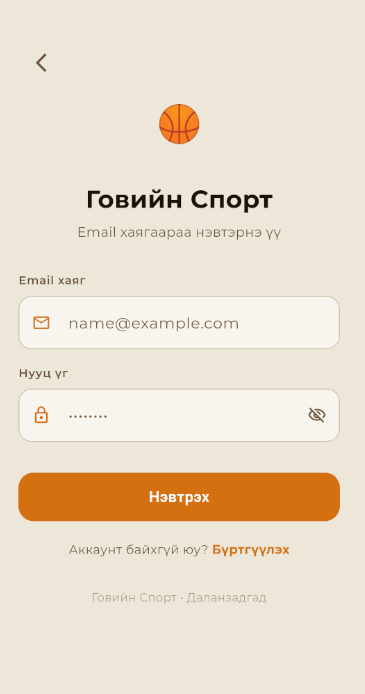
\includegraphics[width=0.35\textwidth]{Figures/screenshot_login.png}
\hspace{1cm}
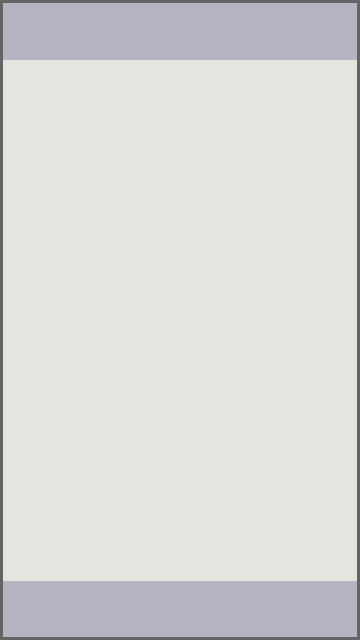
\includegraphics[width=0.35\textwidth]{Figures/screenshot_register.png}
\caption{Нэвтрэх дэлгэц (зүүн) ба бүртгэлийн дэлгэц (баруун)}
\label{fig:screen_auth}
\end{figure}

Email хаяг болон нууц үгээр нэвтрэх дэлгэц нь цайвар бежийн дэвсгэр (\code{\#EDE7DA}) дээр Montserrat фонтоор загварчлагдсан. Бүртгэлийн дэлгэцэд нэр, email, нууц үг оруулах талбарууд байх бөгөөд ``Бүртгүүлэх'' товч дарахад Nodemailer-ийн тусламжтайгаар 6 оронтой баталгаажуулах код илгээгдэнэ.

%-------------------------------------------------------------------------------

\section*{А.2 Нүүр дэлгэц — Спорт заалнуудын жагсаалт}

\begin{figure}[h]
\centering
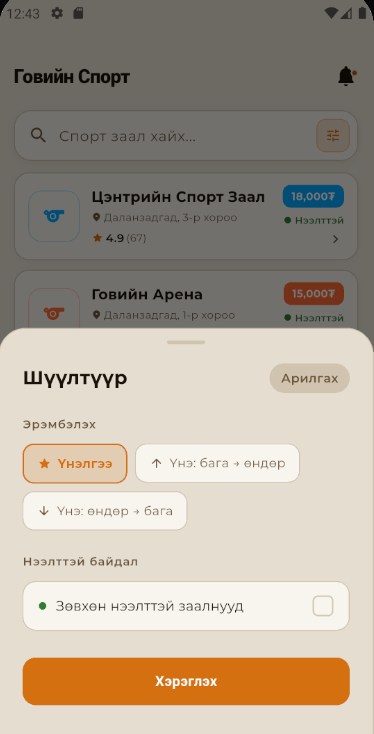
\includegraphics[width=0.35\textwidth]{Figures/screenshot_home.png}
\caption{Нүүр дэлгэц — таван спорт заалны жагсаалт}
\label{fig:screen_home}
\end{figure}

Нүүр дэлгэц нь апп нэвтрэлтийн дараа харагдах анхны дэлгэц юм. Даланзадгадын таван спорт заал картан хэлбэрээр жагсаагдаж, заал бүрийн нэр, байршил, нэг цагийн үнийг харуулна. ``Захиалах'' товч дарахад цагийн хуваарийн дэлгэц нээгдэнэ.

%-------------------------------------------------------------------------------

\section*{А.3 Цагийн хуваарь ба захиалгын дэлгэц}

\begin{figure}[h]
\centering
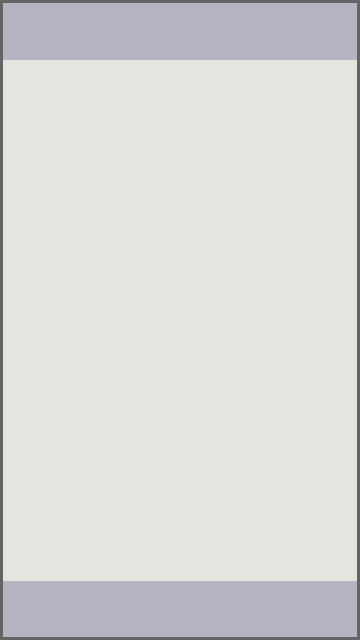
\includegraphics[width=0.35\textwidth]{Figures/screenshot_booking.png}
\hspace{1cm}
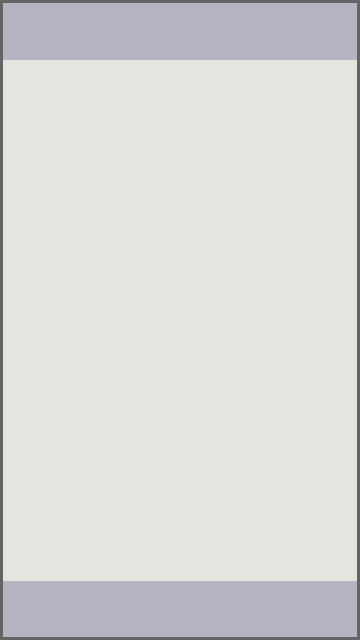
\includegraphics[width=0.35\textwidth]{Figures/screenshot_confirm.png}
\caption{Цагийн хуваарийн дэлгэц (зүүн) ба захиалга баталгаажуулах дэлгэц (баруун)}
\label{fig:screen_booking}
\end{figure}

Цагийн хуваарийн дэлгэцэд сонгосон заал болон огнооны 08:00--00:00 хооронд 16 цагийн үе харагдана. Боломжтой цаг ногоон, захиалагдсан цаг улаан, байгууллагын тогтмол захиалга нил ягаан өнгөөр тэмдэглэгдэнэ. Захиалга баталгаажуулах дэлгэцэд DBK-xxxxx форматын захиалгын код харагдана.

%-------------------------------------------------------------------------------

\section*{А.4 Захиалгын жагсаалт ба AI чатботын дэлгэц}

\begin{figure}[h]
\centering
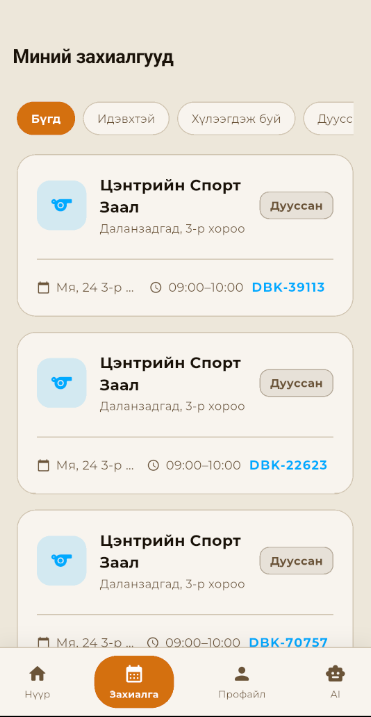
\includegraphics[width=0.35\textwidth]{Figures/screenshot_bookings.png}
\hspace{1cm}
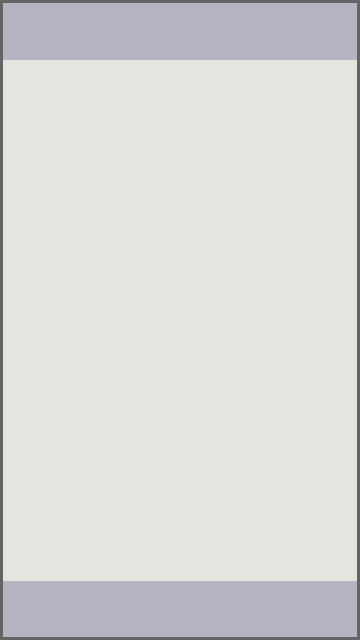
\includegraphics[width=0.35\textwidth]{Figures/screenshot_chat.png}
\caption{Захиалгын жагсаалтын дэлгэц (зүүн) ба AI чатботын дэлгэц (баруун)}
\label{fig:screen_chat}
\end{figure}

Захиалгын дэлгэцэд хэрэглэгчийн бүх захиалга статусаар (идэвхтэй, дууссан, цуцлагдсан) шүүгдэж харагдана. AI чатботын дэлгэцэд Anthropic Claude Haiku болон Groq Llama загваруудаар дамжуулан спорт заалтай холбоотой асуулт асуух боломжтой.

\chapter{Үндсэн тохиргооны файлууд}
\label{AppendixB}
\pagecolor{white}

Энэ хавсралтад системийн байршуулалт болон автоматжуулалттай холбоотой үндсэн тохиргооны файлуудыг оруулав.

%-------------------------------------------------------------------------------

\section*{Б.1 Dockerfile — Node.js/Express бэкэнд}

\begin{lstlisting}[language={}, caption={backend/Dockerfile}]
FROM node:18-alpine
WORKDIR /app
COPY package*.json ./
RUN npm ci --only=production
COPY . .
EXPOSE 3000
CMD ["node", "server.js"]
\end{lstlisting}

Node.js 18 LTS-ийн alpine суурь дүрс ашигласнаар Docker дүрсний хэмжээ хамгийн бага байна. \code{npm ci --only=production} нь зөвхөн production хамаарлуудыг суулгаж, хөгжүүлэлтийн хамаарлуудыг оруулахгүй байлгана.

%-------------------------------------------------------------------------------

\section*{Б.2 GitHub Actions CI/CD Workflow}

\begin{lstlisting}[language={}, caption={.github/workflows/deploy.yml}]
name: Deploy to AWS EC2

on:
  push:
    branches: [main]
    paths:
      - 'backend/**'

jobs:
  deploy:
    runs-on: ubuntu-latest
    steps:
      - uses: actions/checkout@v3

      - name: Configure AWS credentials
        uses: aws-actions/configure-aws-credentials@v2
        with:
          aws-access-key-id: ${{ secrets.AWS_ACCESS_KEY_ID }}
          aws-secret-access-key: ${{ secrets.AWS_SECRET_ACCESS_KEY }}
          aws-region: ap-northeast-1

      - name: Login to Amazon ECR
        id: login-ecr
        uses: aws-actions/amazon-ecr-login@v1

      - name: Build and push Docker image
        env:
          ECR_REGISTRY: ${{ steps.login-ecr.outputs.registry }}
          IMAGE_TAG: ${{ github.sha }}
        run: |
          docker build \
            -t $ECR_REGISTRY/dz-zaal-backend:$IMAGE_TAG \
            -t $ECR_REGISTRY/dz-zaal-backend:latest \
            ./backend
          docker push $ECR_REGISTRY/dz-zaal-backend:$IMAGE_TAG
          docker push $ECR_REGISTRY/dz-zaal-backend:latest

      - name: Deploy to EC2
        uses: appleboy/ssh-action@master
        with:
          host: ${{ secrets.EC2_HOST }}
          username: ubuntu
          key: ${{ secrets.EC2_SSH_KEY }}
          script: |
            aws ecr get-login-password --region ap-northeast-1 | \
              docker login --username AWS --password-stdin \
              ${{ secrets.ECR_REGISTRY }}
            docker pull ${{ secrets.ECR_REGISTRY }}/dz-zaal-backend:latest
            docker stop dz-zaal-backend || true
            docker rm dz-zaal-backend || true
            docker run -d --name dz-zaal-backend \
              -p 3000:3000 \
              --env-file /home/ubuntu/.env \
              ${{ secrets.ECR_REGISTRY }}/dz-zaal-backend:latest
\end{lstlisting}

Workflow нь \code{backend/} хавтаст өөрчлөлт push хийх үед автоматаар ажиллана. AWS нэвтрэлтийн мэдээлэл (access key, SSH түлхүүр) нь GitHub Secrets-д хадгалагдаж кодод задрахгүй.

%-------------------------------------------------------------------------------

\section*{Б.3 Firebase Firestore Security Rules}

\begin{lstlisting}[language={}, caption={firestore.rules}]
rules_version = '2';
service cloud.firestore {
  match /databases/{database}/documents {

    match /users/{userId} {
      allow read, write: if request.auth != null
                         && request.auth.uid == userId;
    }

    match /bookings/{bookingId} {
      allow read: if request.auth != null
                  && resource.data.userId == request.auth.uid;
      allow create: if request.auth != null;
      allow update, delete: if request.auth != null
                             && resource.data.userId == request.auth.uid;
    }

    match /fixed_bookings/{docId} {
      allow read: if request.auth != null;
      allow write: if false;
    }

    match /email_verifications/{docId} {
      allow read, write: if false;
    }
  }
}
\end{lstlisting}

Firestore аюулгүй байдлын дүрэм нь хэрэглэгч зөвхөн өөрийн захиалгыг унших, засах эрхтэй болохыг баталгаажуулна. \code{email\_verifications} болон \code{fixed\_bookings} цуглуулгуудад клиент тал бичих боломжгүй.


%-------------------------------------------------------------------------------
%	BIBLIOGRAPHY
%-------------------------------------------------------------------------------
\defformat % Бүлгийн нэрийг оргиналь байдлаар хэвлэх

\addchaptertocentry{Ном зүй} % Ном зүйг гарчигт нэмэх

\printbibliography[heading=bibliography,title={Ном зүй}]

%-------------------------------------------------------------------------------

\end{document}  
 